\chapter{Model evaluation}
\label{cha:Model evaluation}

This chapter discusses the performance of the models that were introduced in Chapter \ref{cha:Forecasting the daily electricity consumption} on the test set. As was shown in Table \ref{tab:summ_data}, the test set consists out of the days of the month December. The goal of the test set is to assess the model performance on new data and it therefore important that the models are not trained and their parameters are not tuned with data coming from the test set. Missing days in the test set are removed to avoid the influence of the estimation error of the reference signal on the model performance. In this chapter first the model selection is explained after which a discussion of the performance on the test set follows.

\section{Model selection}\label{s:Model selection}
From Chapter \ref{cha:Forecasting the daily electricity consumption} the model parameters are tuned, but there is still a factor of random model performance due to the random initialization of the weight matrices. To reduce this influence, the model is trained $ 10 $ times and the model that performed best on a validation set using the $ MAE $ metric is selected. As validation set the $ 10 $ last days of November are used. Also, during the training early stopping is applied wherefore an additional $ 10\% $ of the training data is taken to serve as a second validation set. For a stateless model this $ 10\% $ is randomly taken from the remaining training matrix. For a stateful model this $ 10\% $ originates form the end of the training matrix. The patience parameter is taken as $ 5 $, which means that the validation error can increase $ 5 $ times before the model is stopped. The maximum amount of epochs that is allowed is $ 150 $. The values of the parameters for each of the three time series can be found in Chapter \ref{cha:Forecasting the daily electricity consumption}. Table \ref{tab:summ_model_selection} summarizes the amount of epochs that the model that is finally selected has run.

\begin{table}[h]
	\centering
	\begin{tabular}{@{}l|ccc@{}} \toprule
				         & \textbf{Model $ 1 $} & \textbf{Model $ 2 $} & \textbf{Model $ 3 $}\\\midrule
		\textbf{Serie 1} & $5 $&$ 16$  & $5 $\\
		\textbf{Serie 2} & $7 $&$ 150 $  & $150$\\
		\textbf{Serie 3} & $19 $&$ 11 $  & $6$\\\bottomrule
	\end{tabular}
	\caption{The amount of training epochs that each model has trained on the different series.}
	\label{tab:summ_model_selection}
\end{table}



\subsubsection{Performance on the test set}
In this section the results on the test set are discussed for the models that were selected in section \ref{s:Model selection}. 
Also the two best baseline models ``mean forecast'' and ``MAPE forecast'' that were explained in Section \ref{s:Baseline models} are included in the comparison. An advantage that the baseline models have in comparison to the LSTM neural networks is that they use the previous data till the day to forecast to make predictions while the LSTM neural networks only trains on the input time series till November. This is because it needs data for the validation set to tune parameters and implement early stopping. The baseline models and the LSTM neural networks both belong to a different group of models respectively the lazy models and eager models. A lazy model only looks at the data when the query is known e.g. what day to forecast and to the contrary an eager model already makes generalizations on the training set before it knows which day it has to predict for.\\








To get a better feeling of the actual output of the different models, Figure \ref{fig:individual_days_prediction} shows the prediction of the different models on a chosen day in the test set.
 
 \begin{figure}[ht]
 	\begin{subfigure}{0.32\textwidth}
 		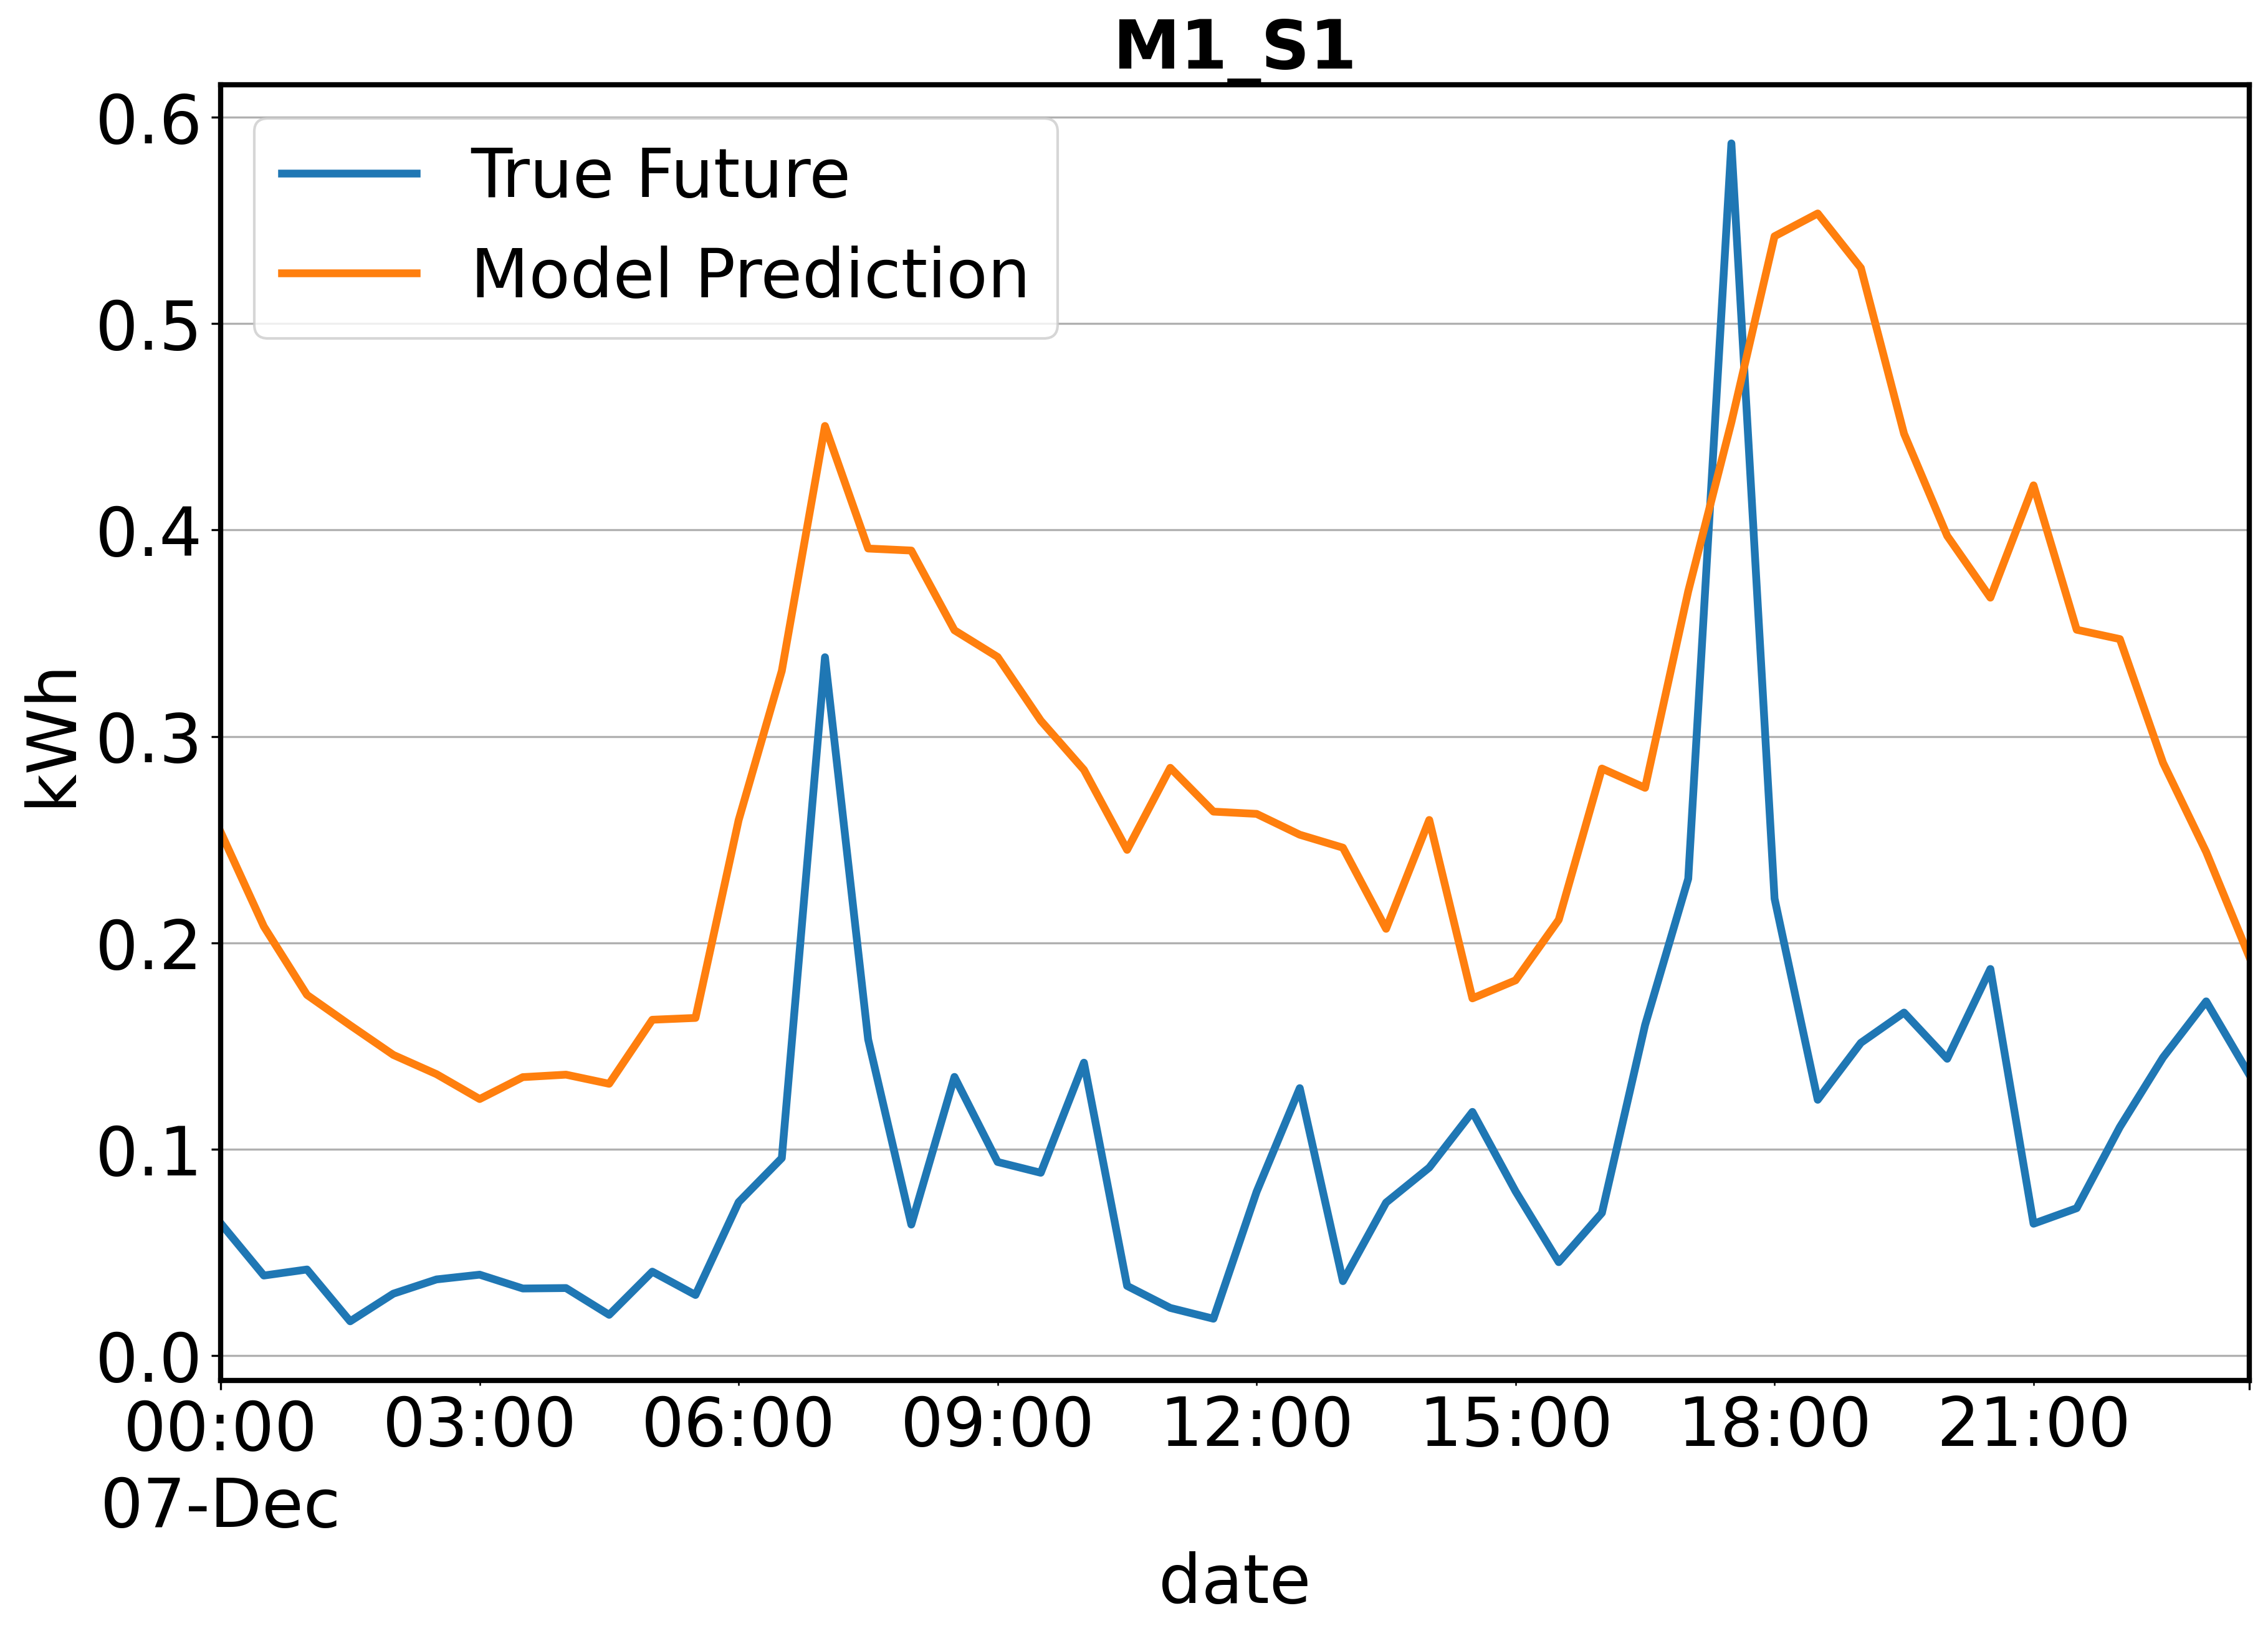
\includegraphics[width=1\linewidth]{IDM1_S1_Day341.png}
 		\caption{Model $ 1 $ - Serie $ 1 $}
 	\end{subfigure}	 	
 	\begin{subfigure}{0.32\textwidth}
 		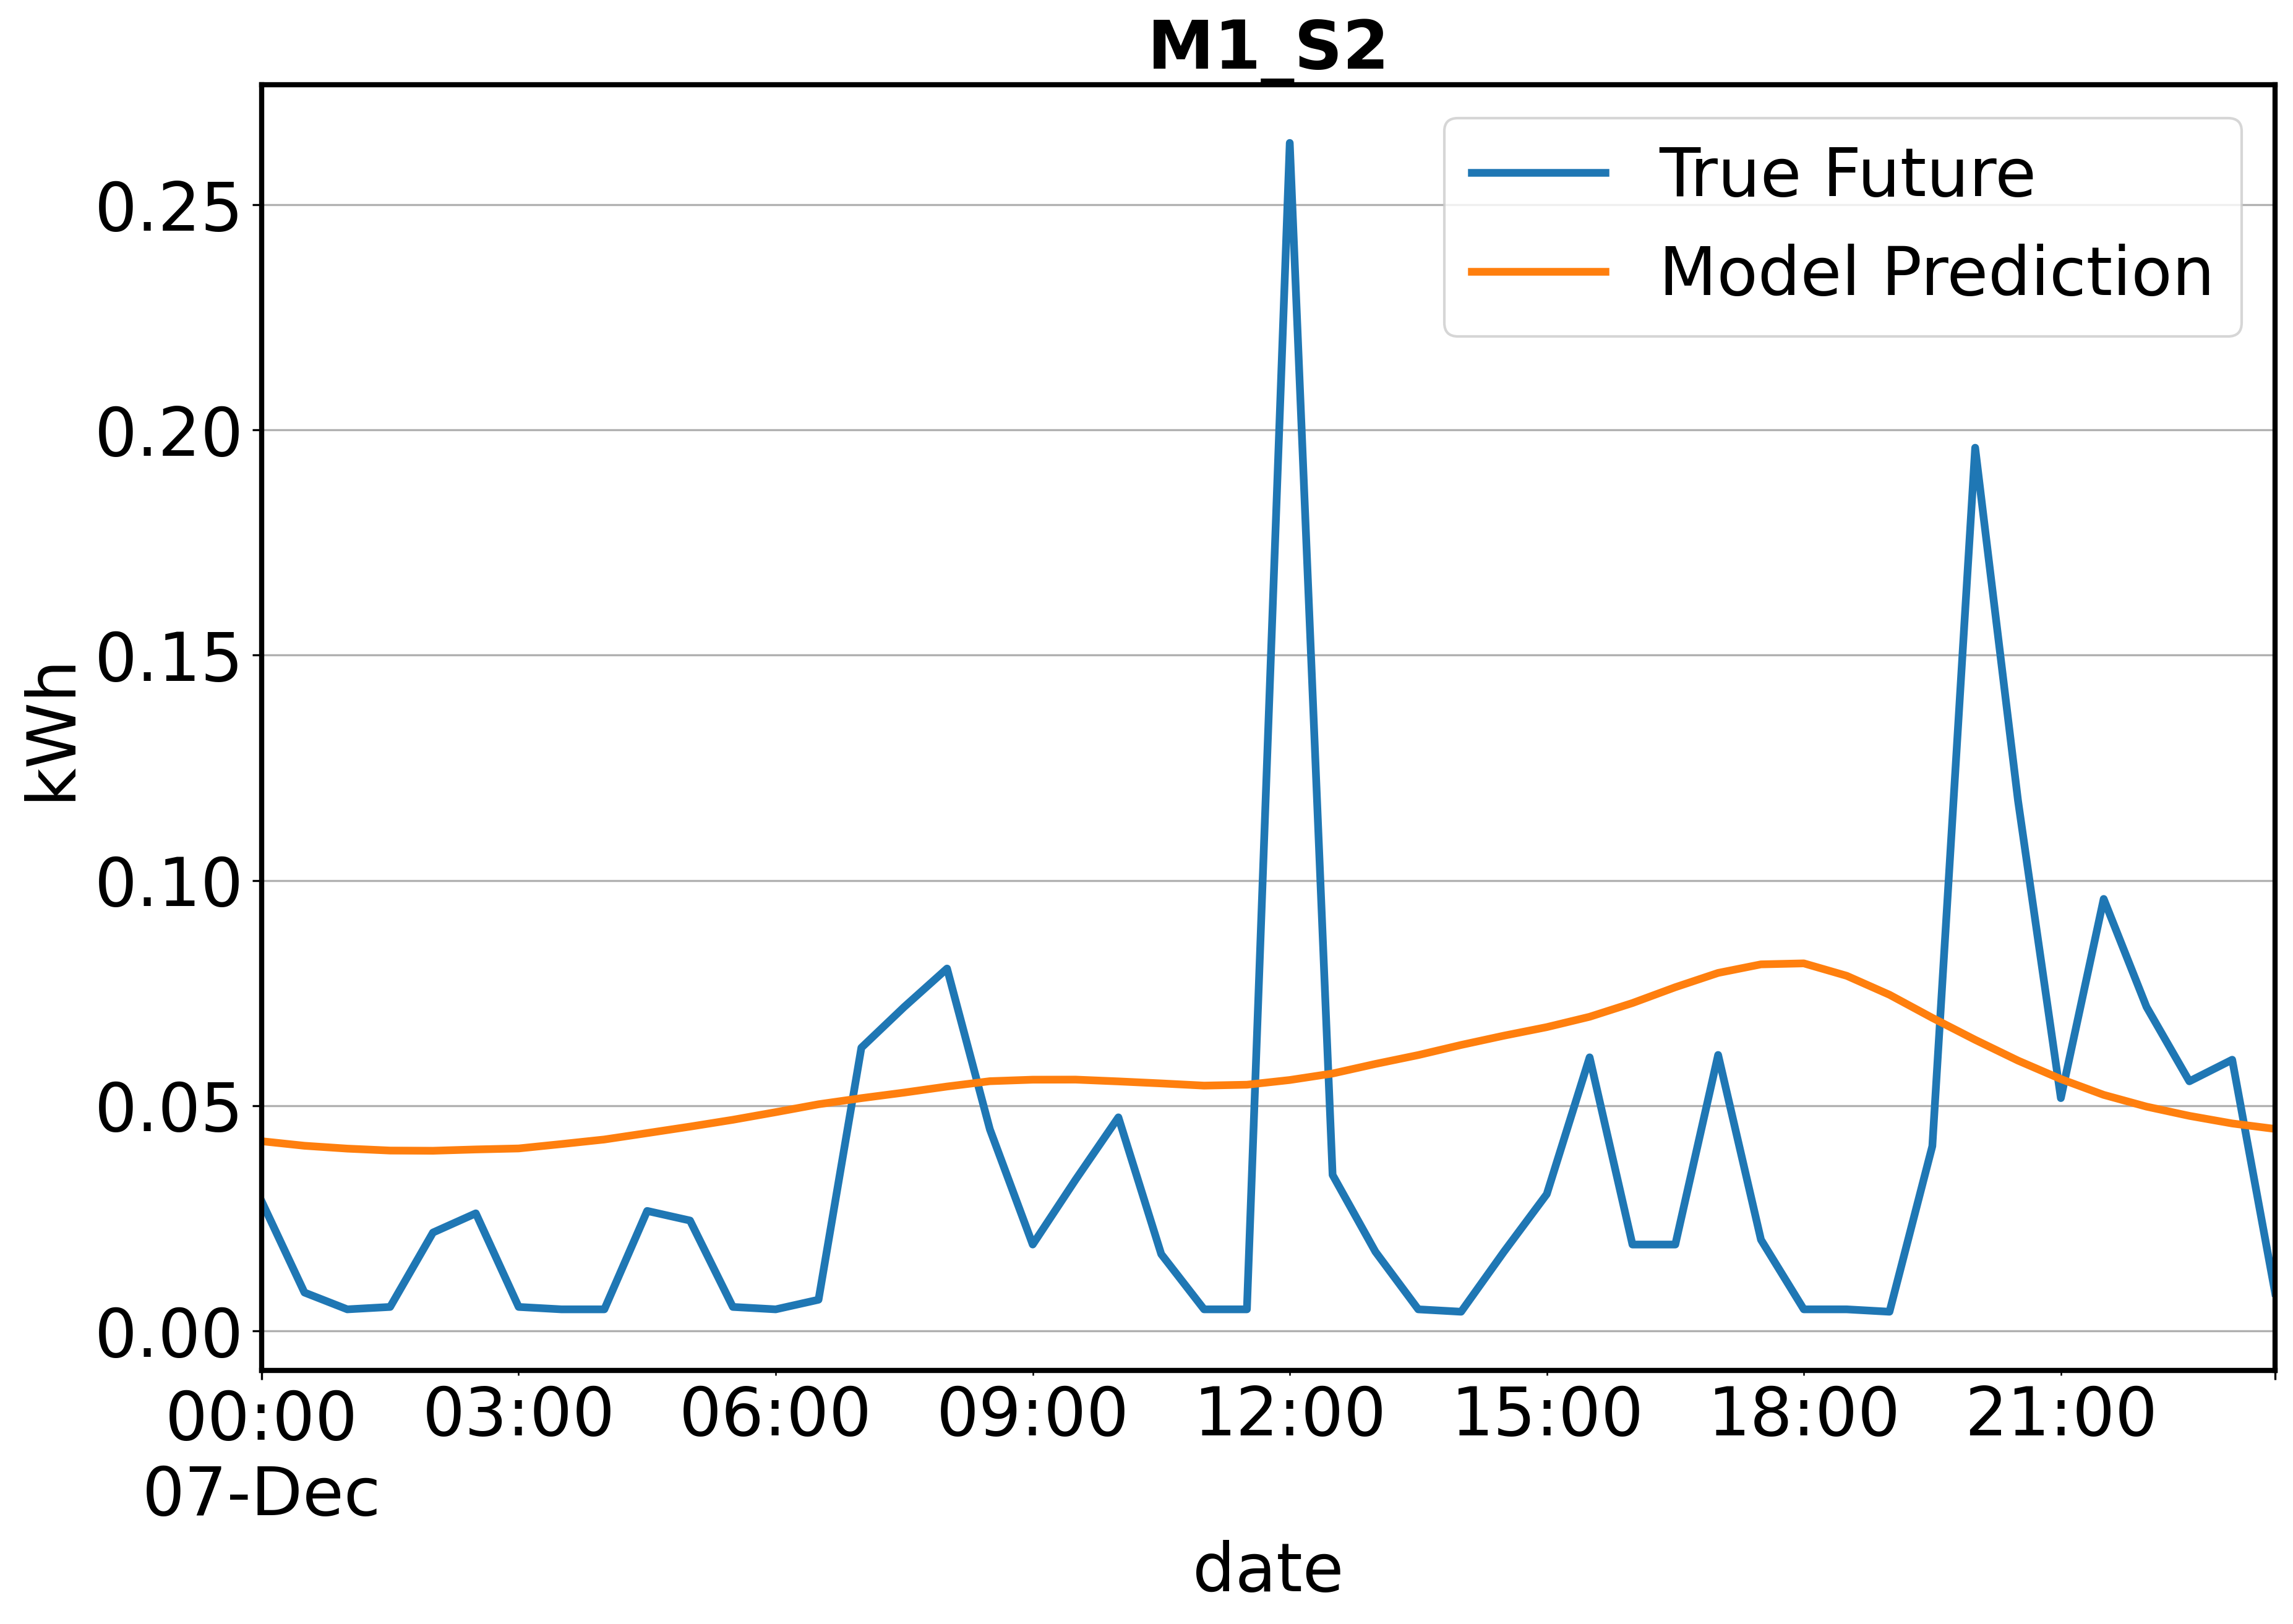
\includegraphics[width=1\linewidth]{IDM1_S2_Day341.png}
 		\caption{Model $ 1 $ - Serie $ 2 $}
 	\end{subfigure}	
 	\begin{subfigure}{0.32\textwidth}
 		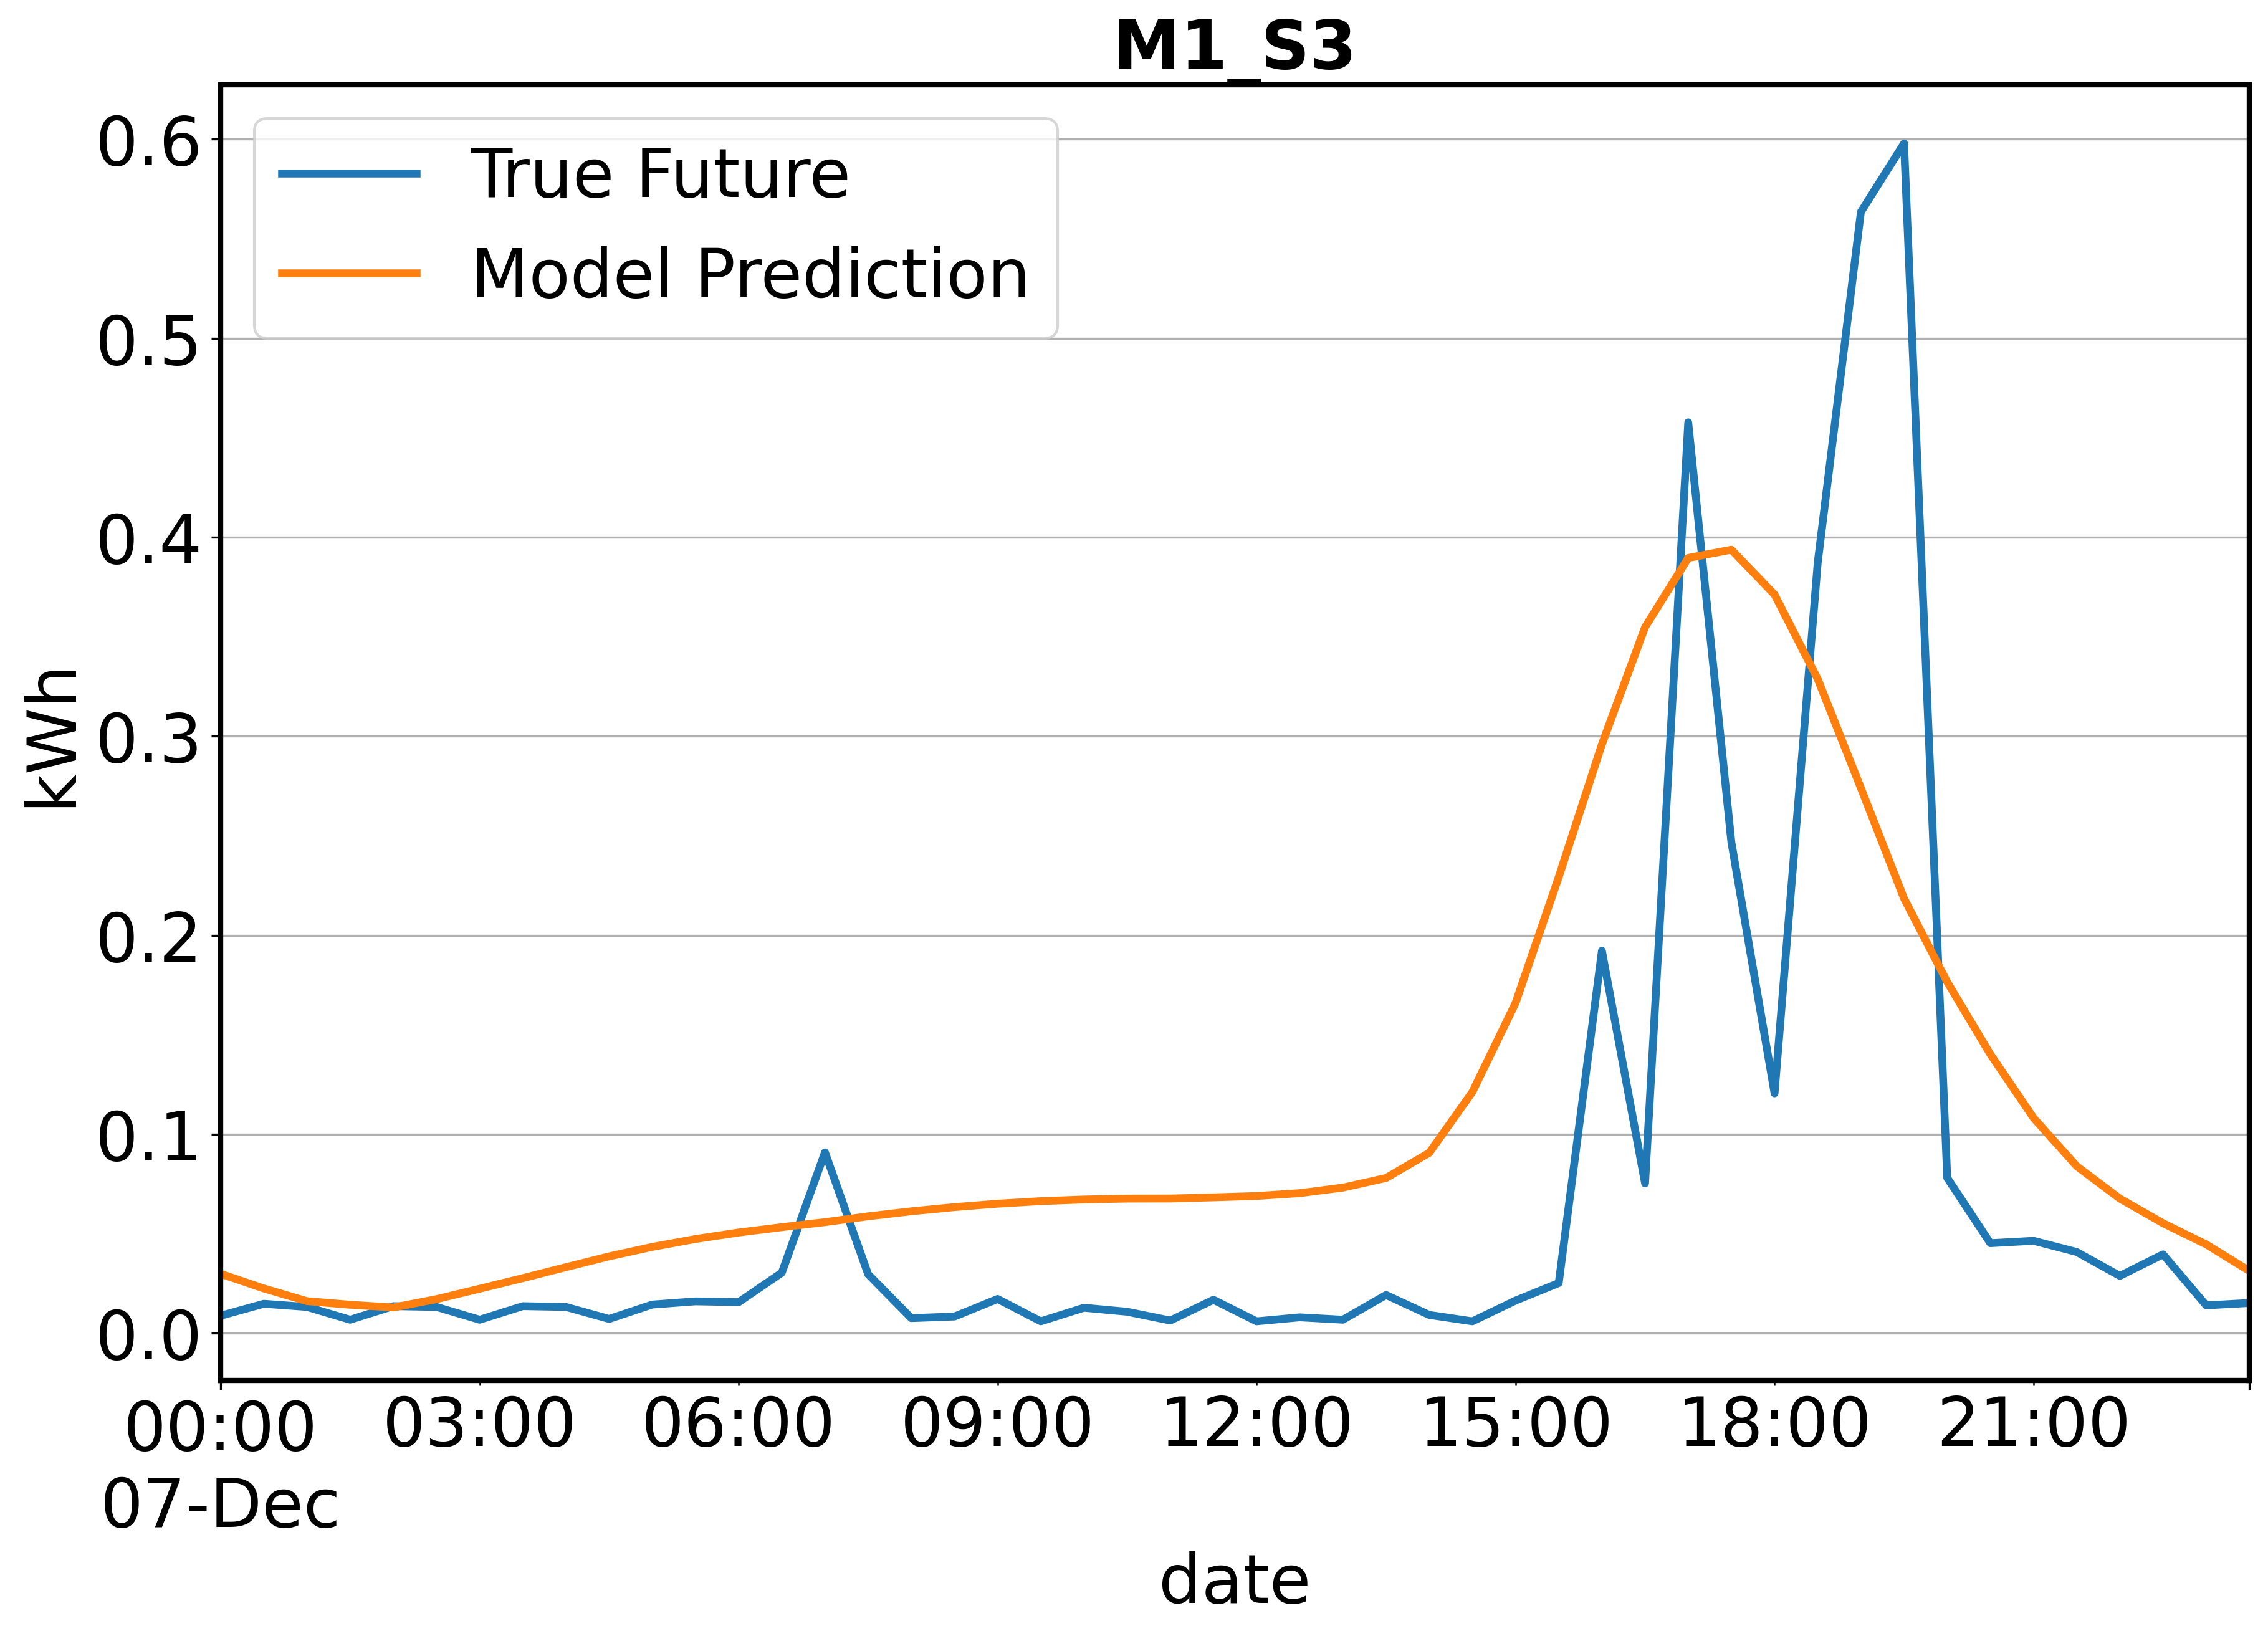
\includegraphics[width=1\linewidth]{IDM1_S3_Day341.png}
 		\caption{Model $ 1 $ - Serie $ 3 $}
 	\end{subfigure}
  	\begin{subfigure}{0.32\textwidth}
 		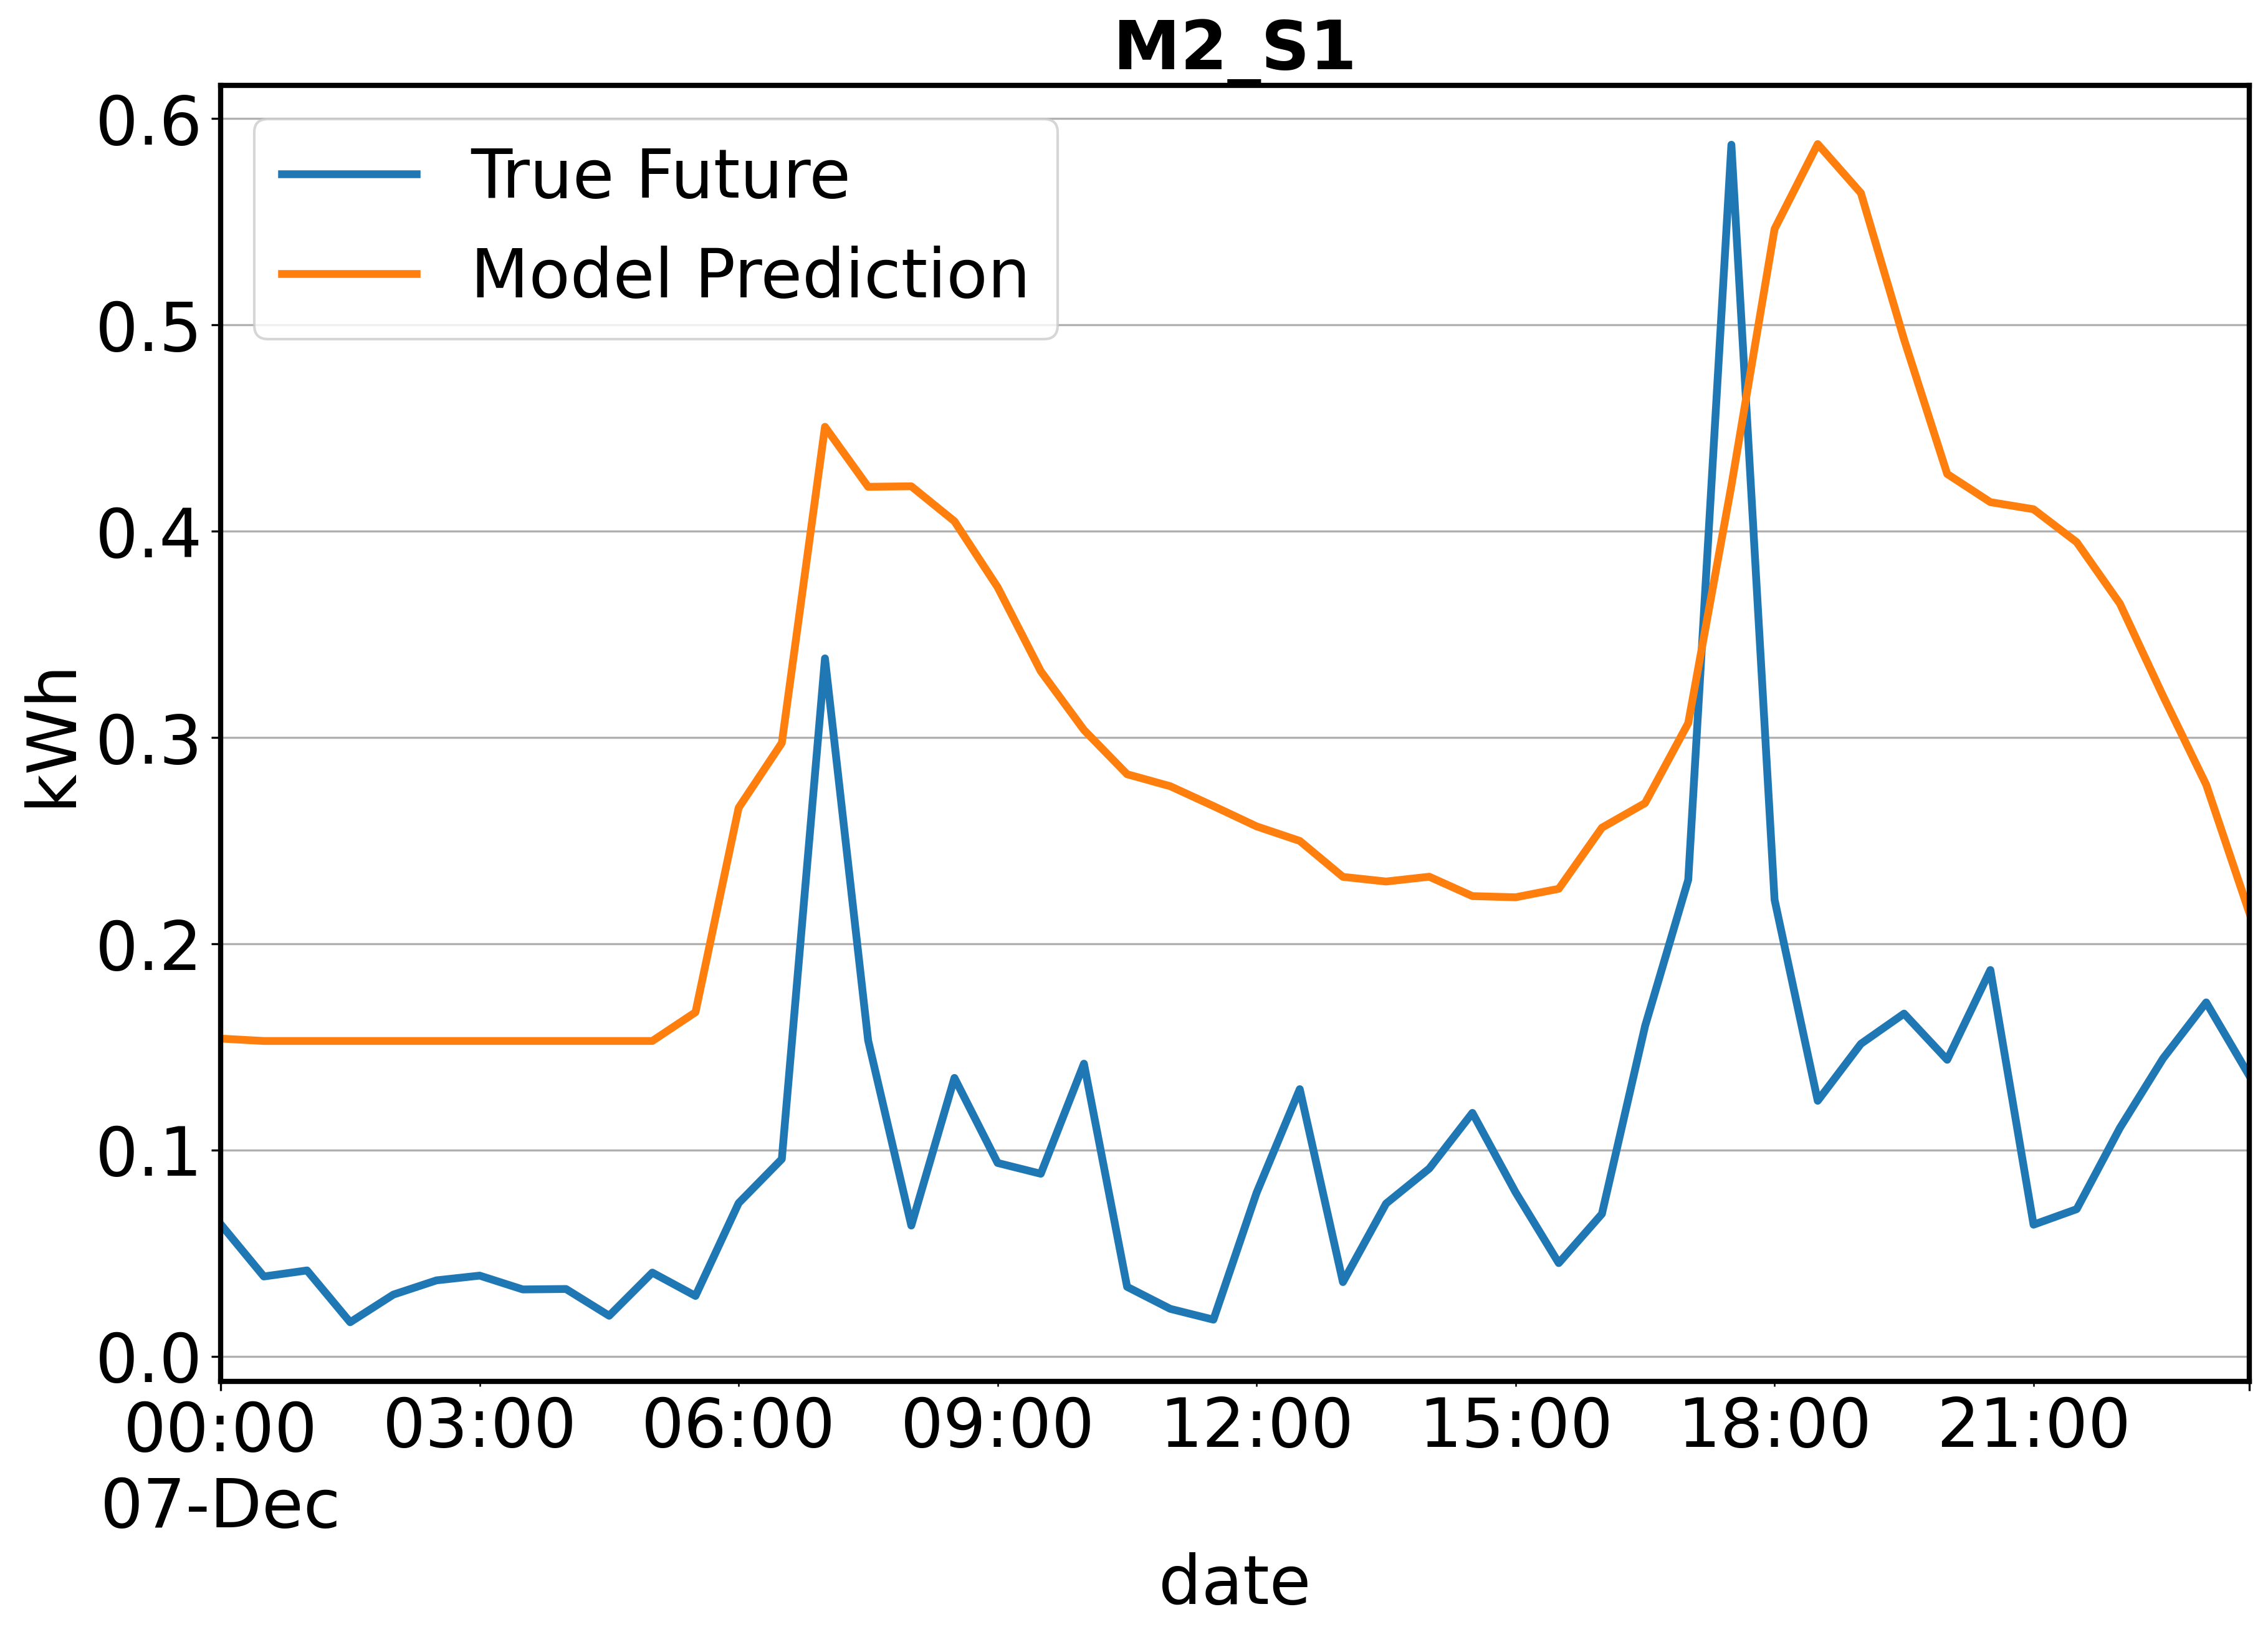
\includegraphics[width=1\linewidth]{IDM2_S1_Day341.png}
 		\caption{Model $ 2 $ - Serie $ 1 $}
 	\end{subfigure}	 	
	 \begin{subfigure}{0.32\textwidth}
	 	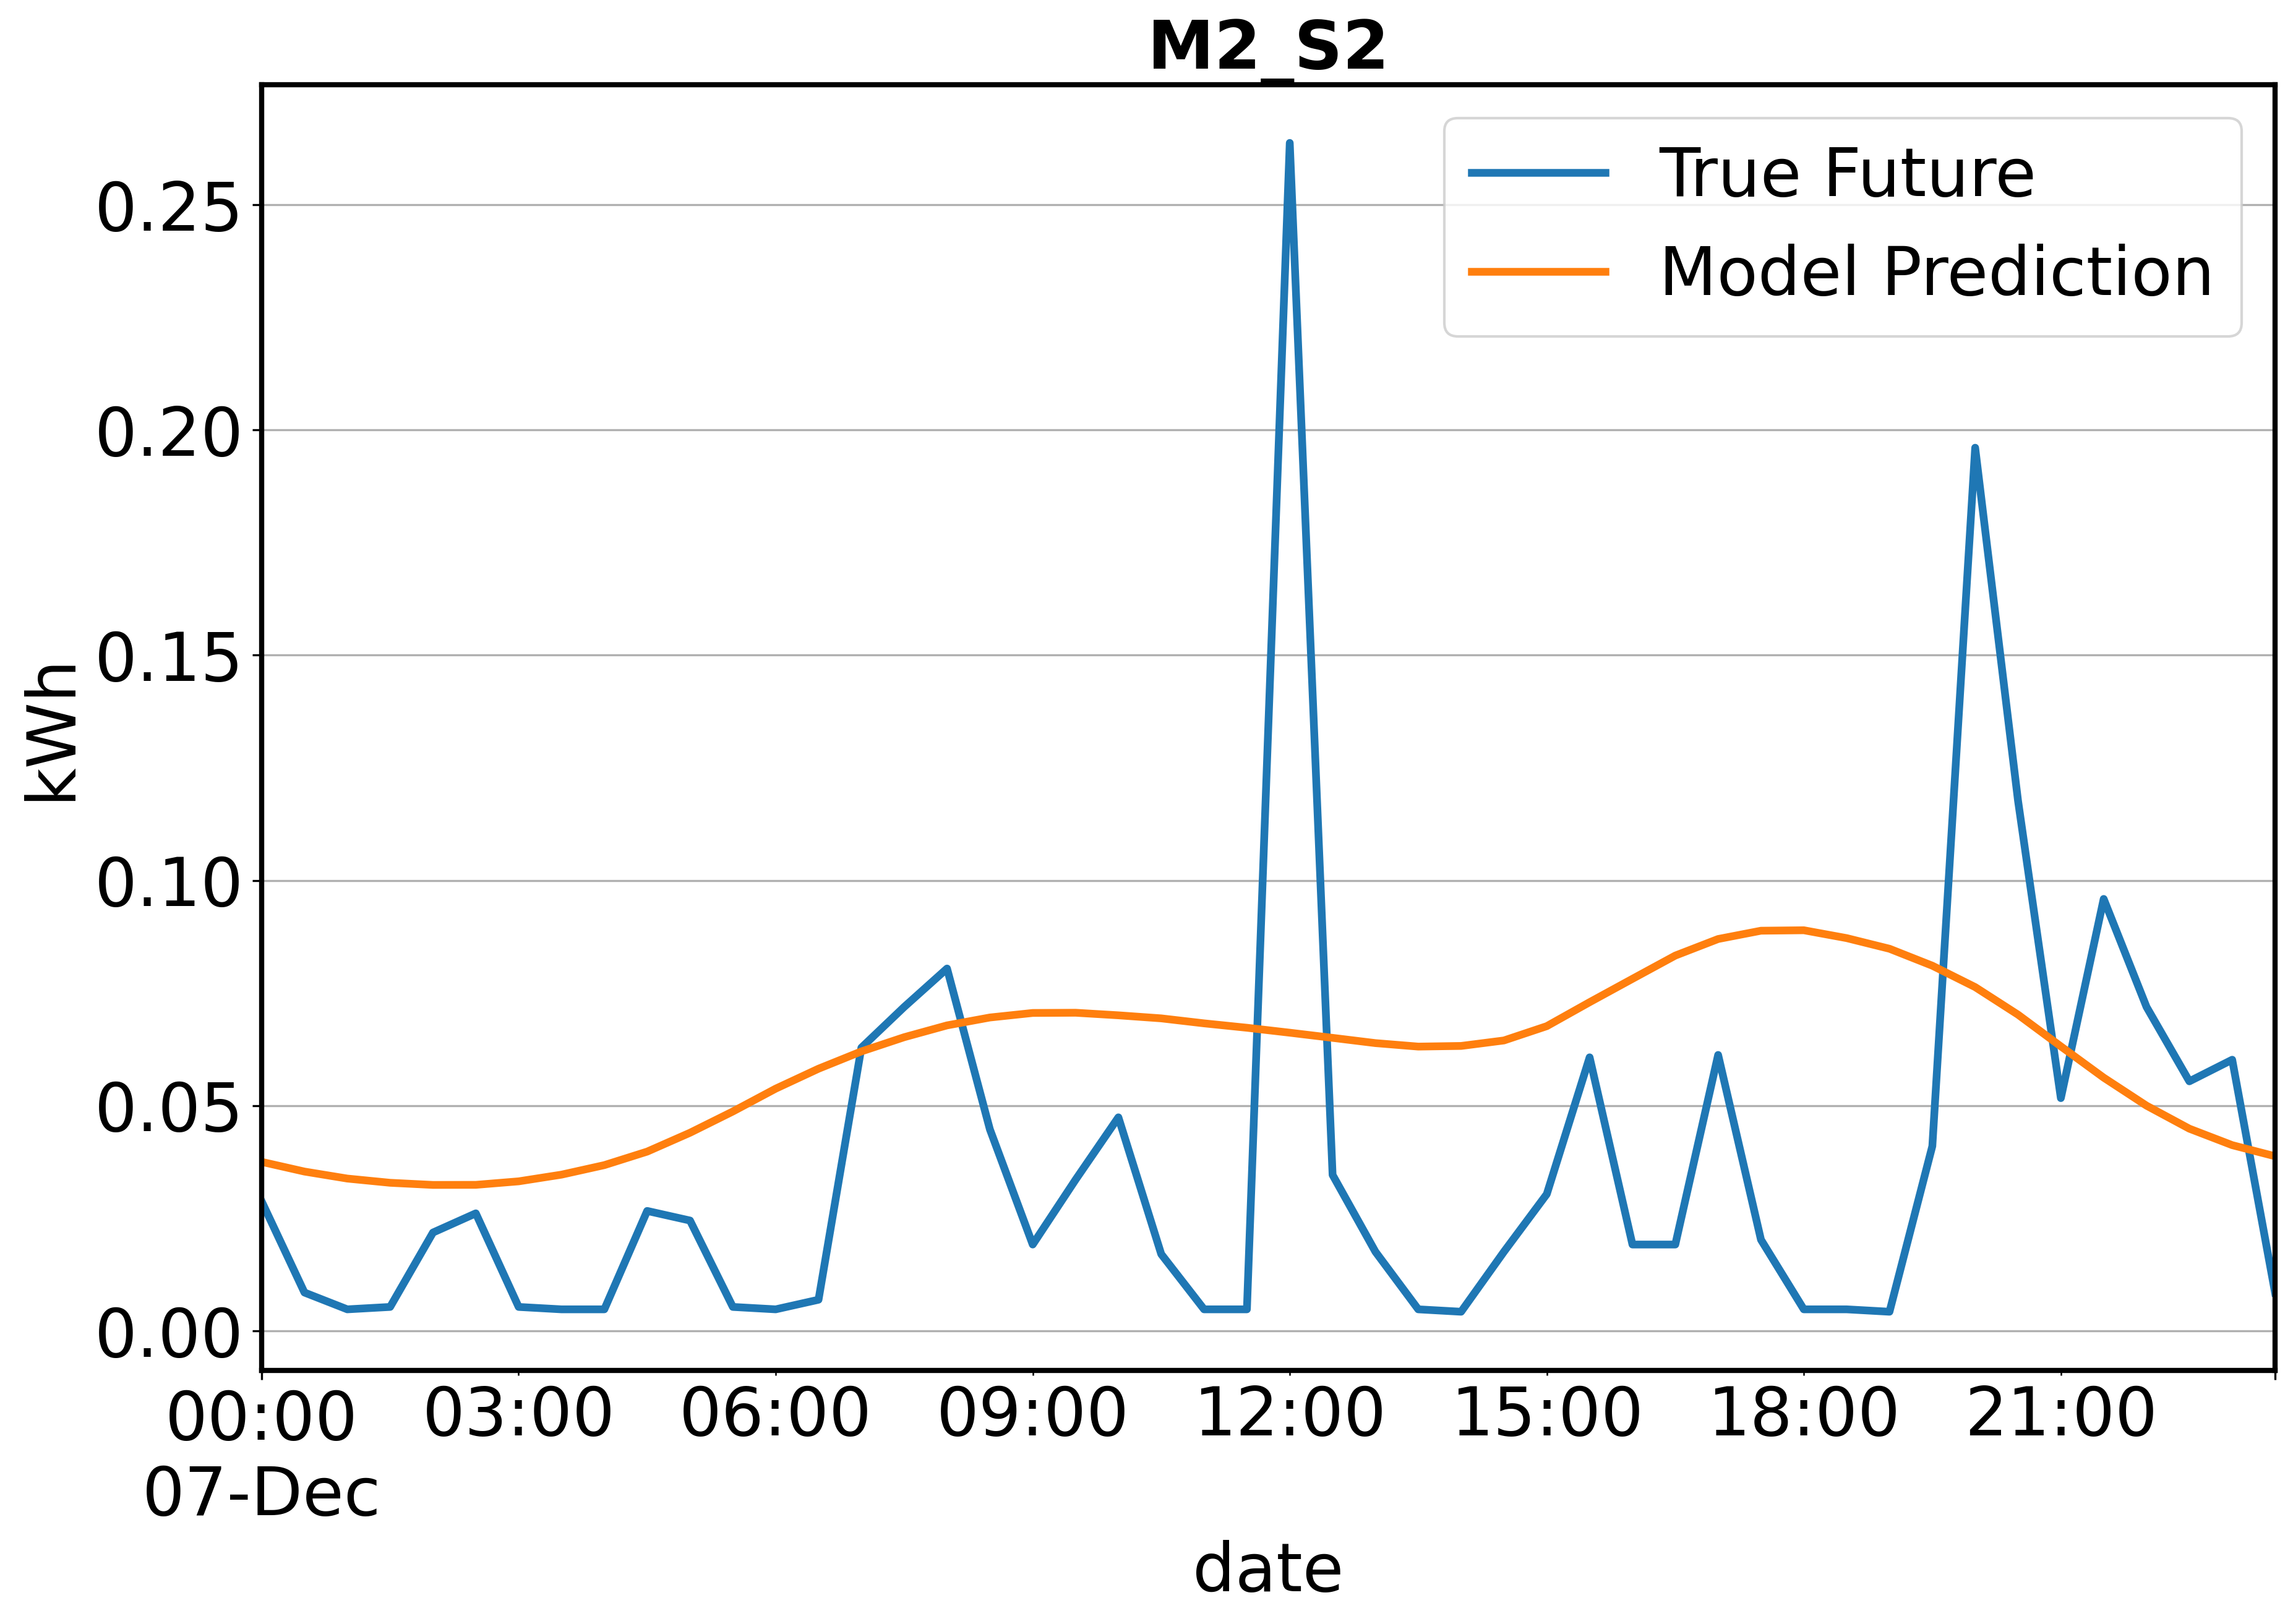
\includegraphics[width=1\linewidth]{IDM2_S2_Day341.png}
	 	\caption{Model $ 2 $ - Serie $ 2 $}
	 \end{subfigure}	
	 \begin{subfigure}{0.32\textwidth}
	 	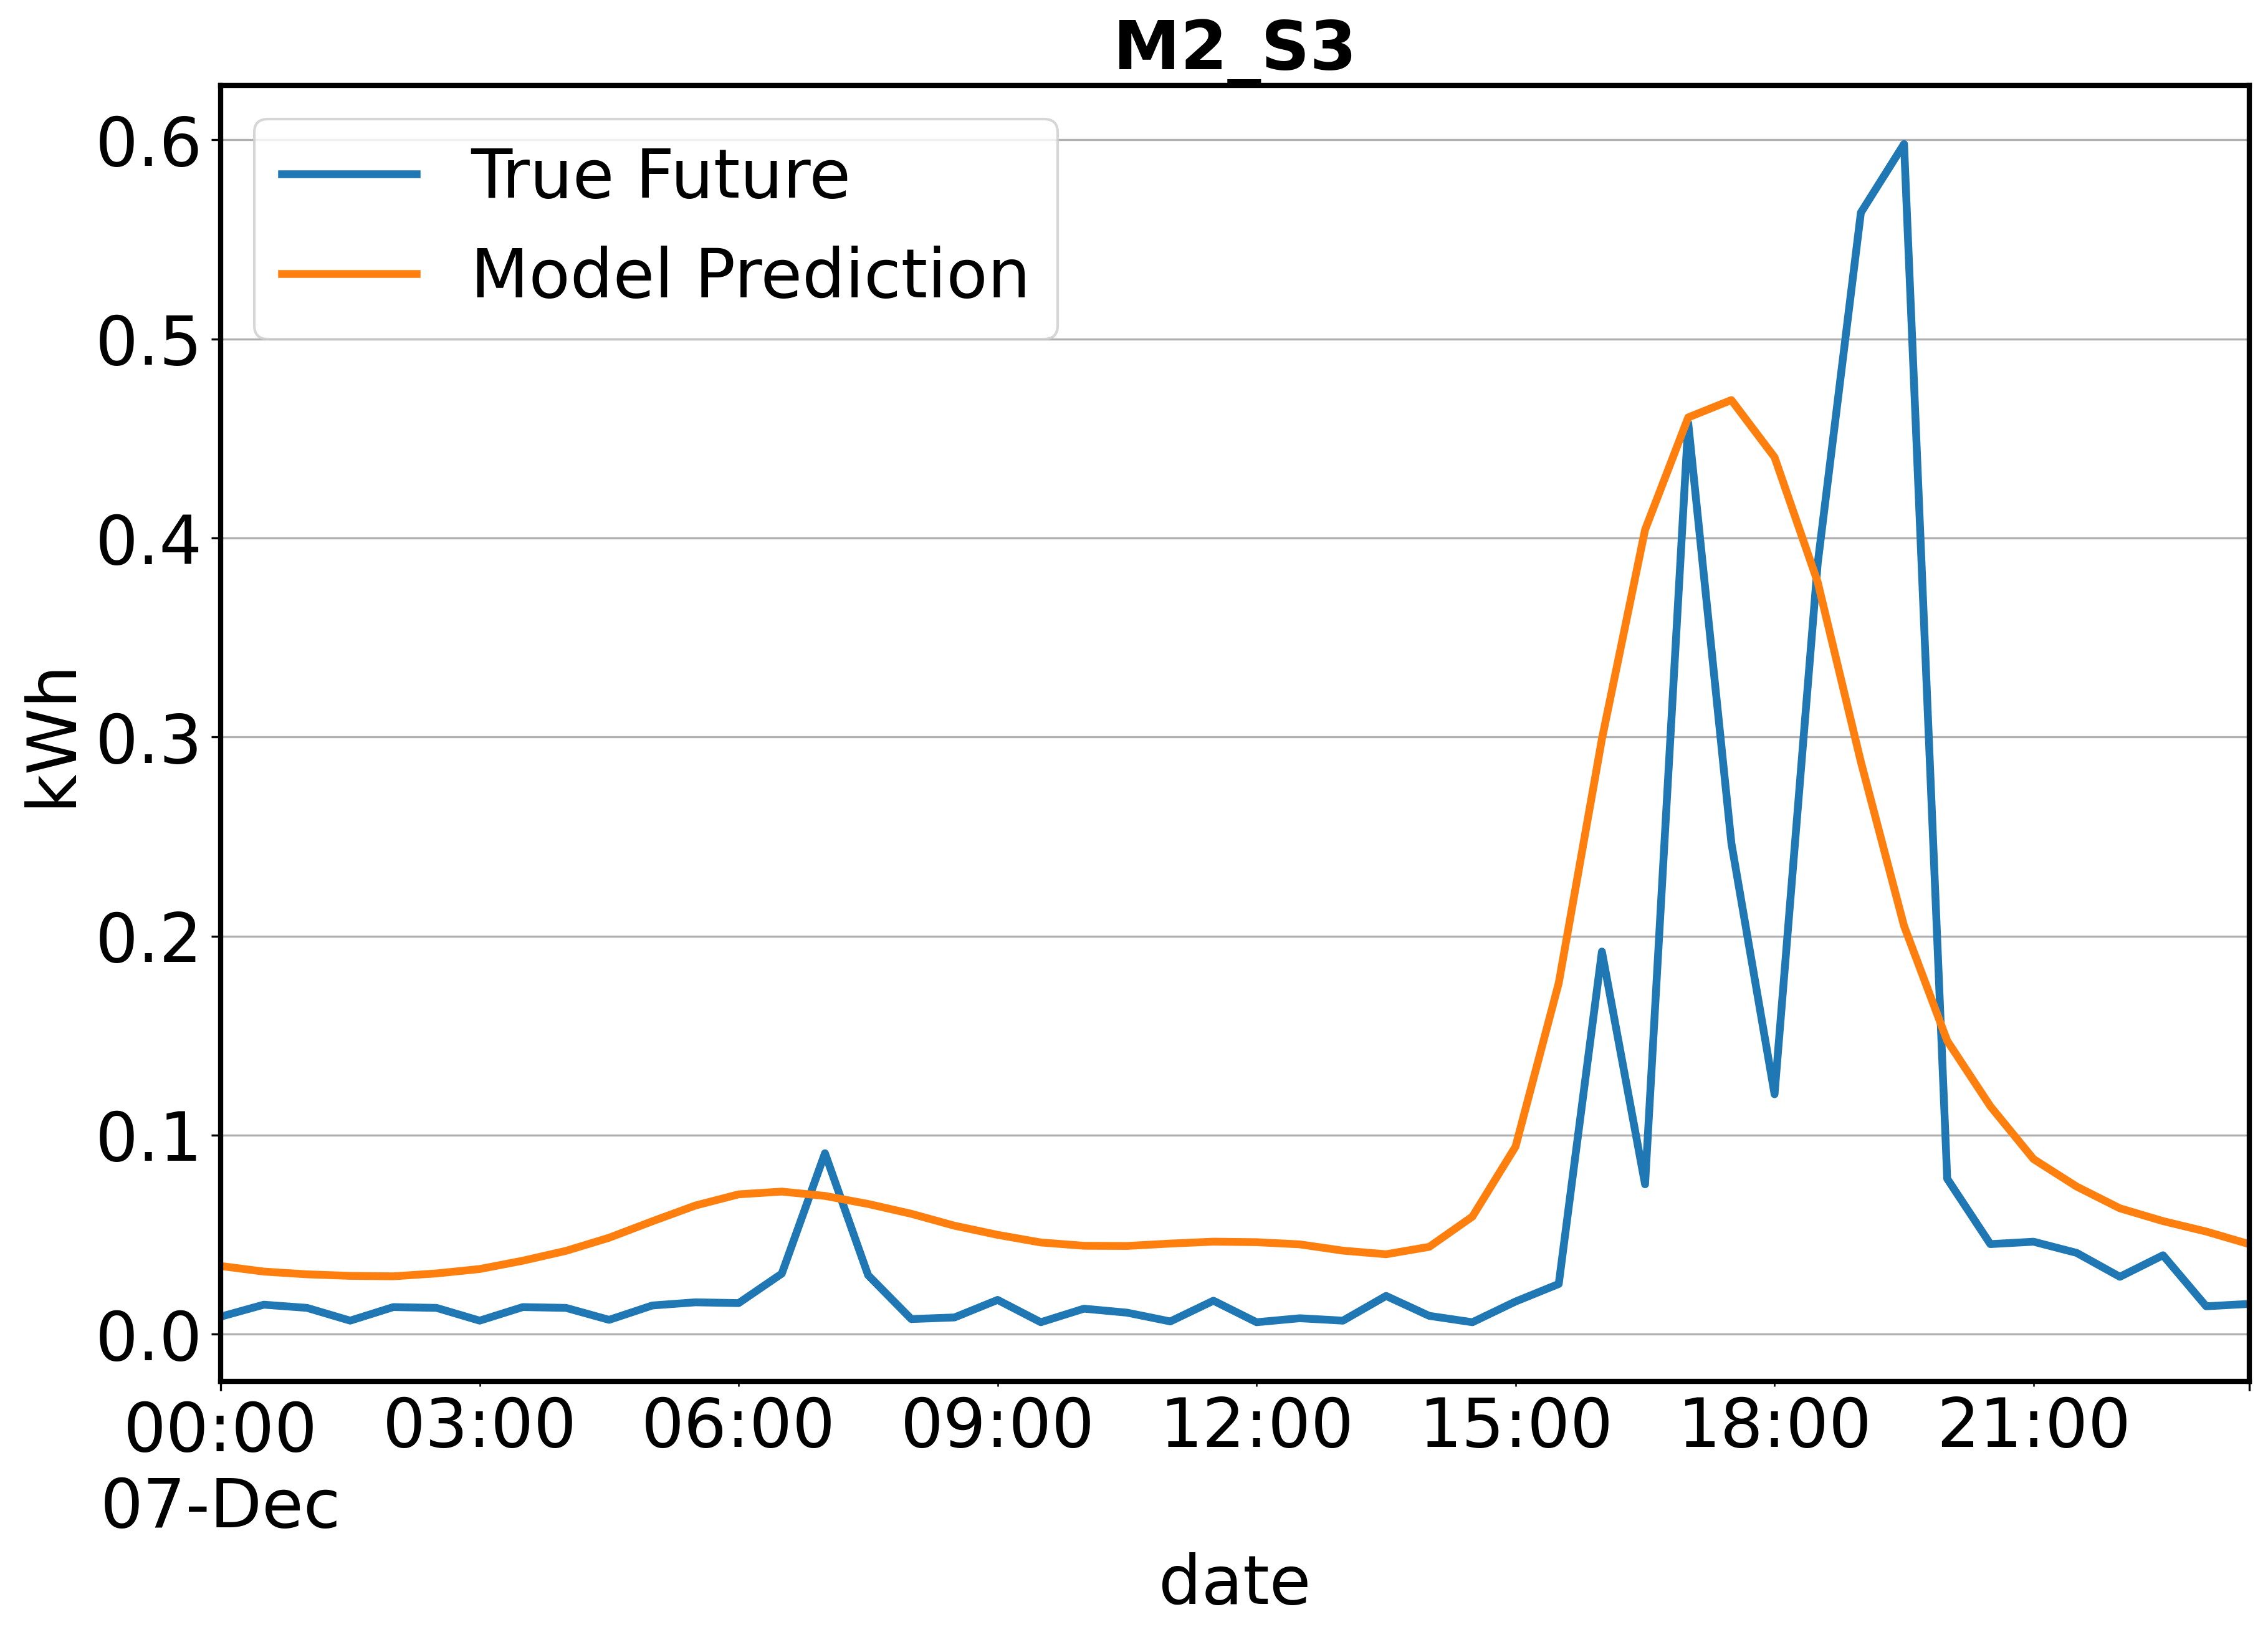
\includegraphics[width=1\linewidth]{IDM2_S3_Day341.png}
	 	\caption{Model $ 2 $ - Serie $ 3 $}
	 \end{subfigure}
 	\begin{subfigure}{0.32\textwidth}
	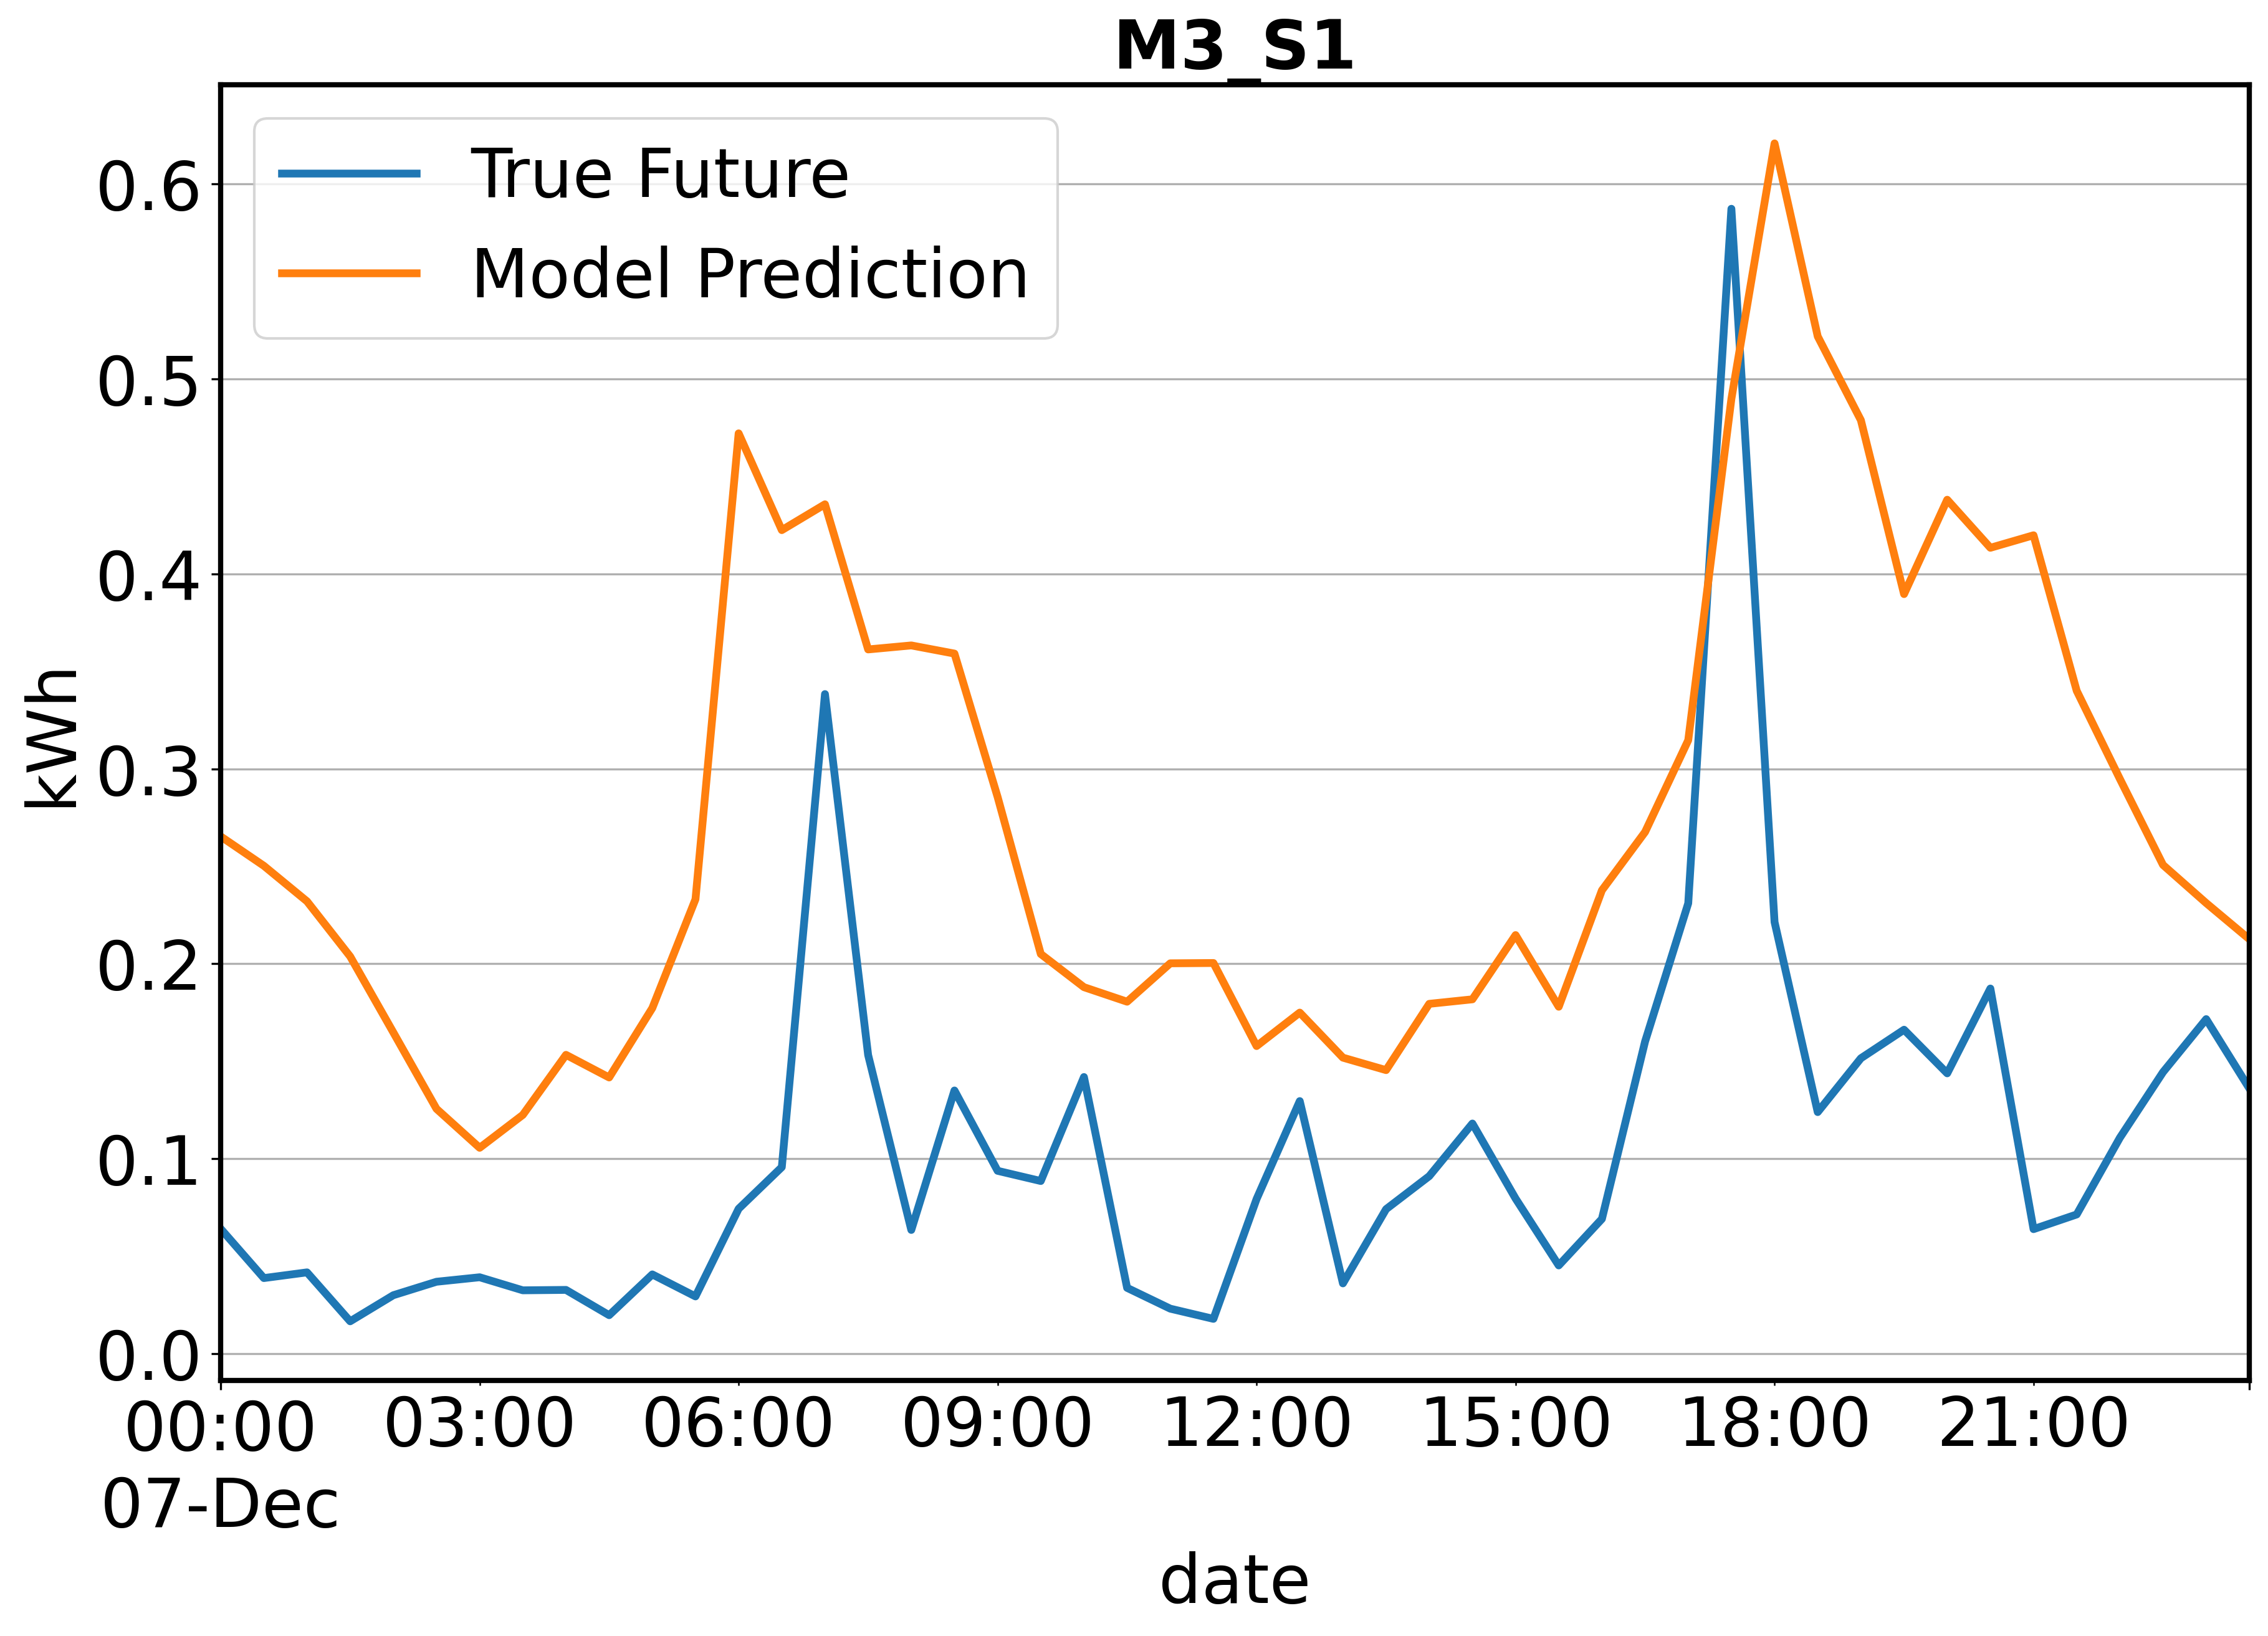
\includegraphics[width=1\linewidth]{IDM3_S1_Day341.png}
	\caption{Model $3 $ - Serie $ 1 $}
	\end{subfigure}	 	
	\begin{subfigure}{0.32\textwidth}
		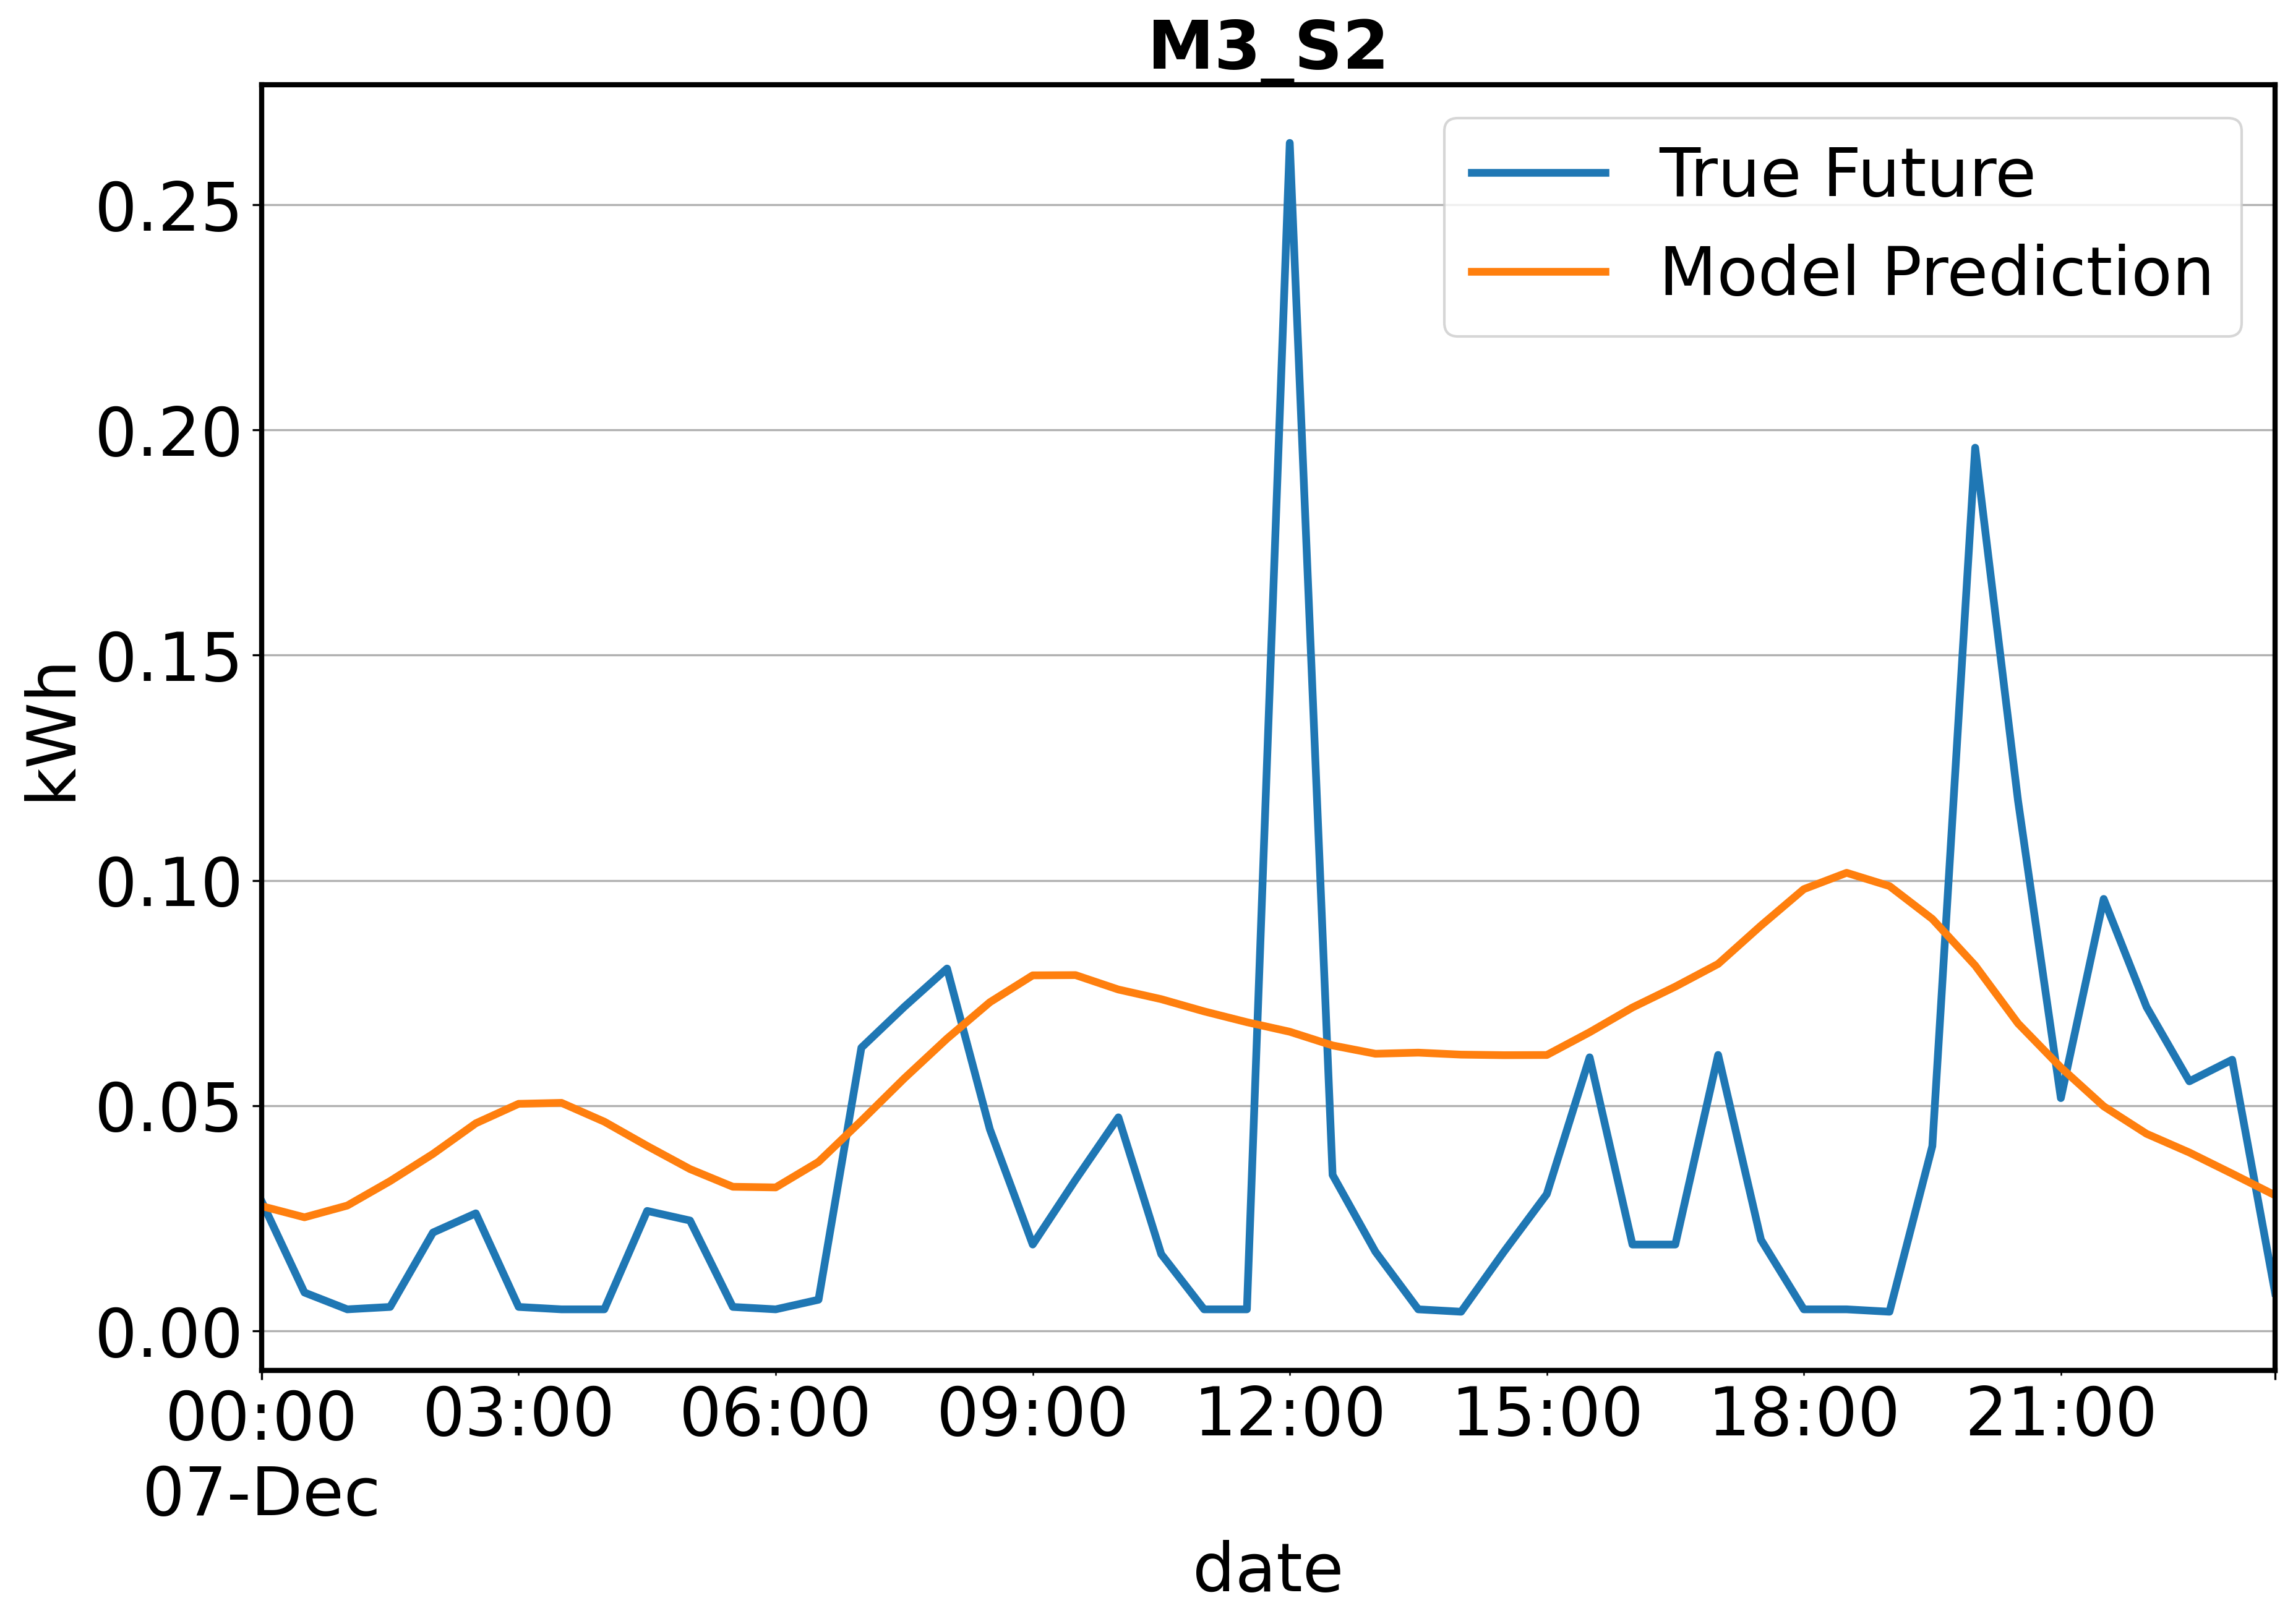
\includegraphics[width=1\linewidth]{IDM3_S2_Day341.png}
		\caption{Model $3 $ - Serie $ 2 $}
	\end{subfigure}	
	\begin{subfigure}{0.32\textwidth}
		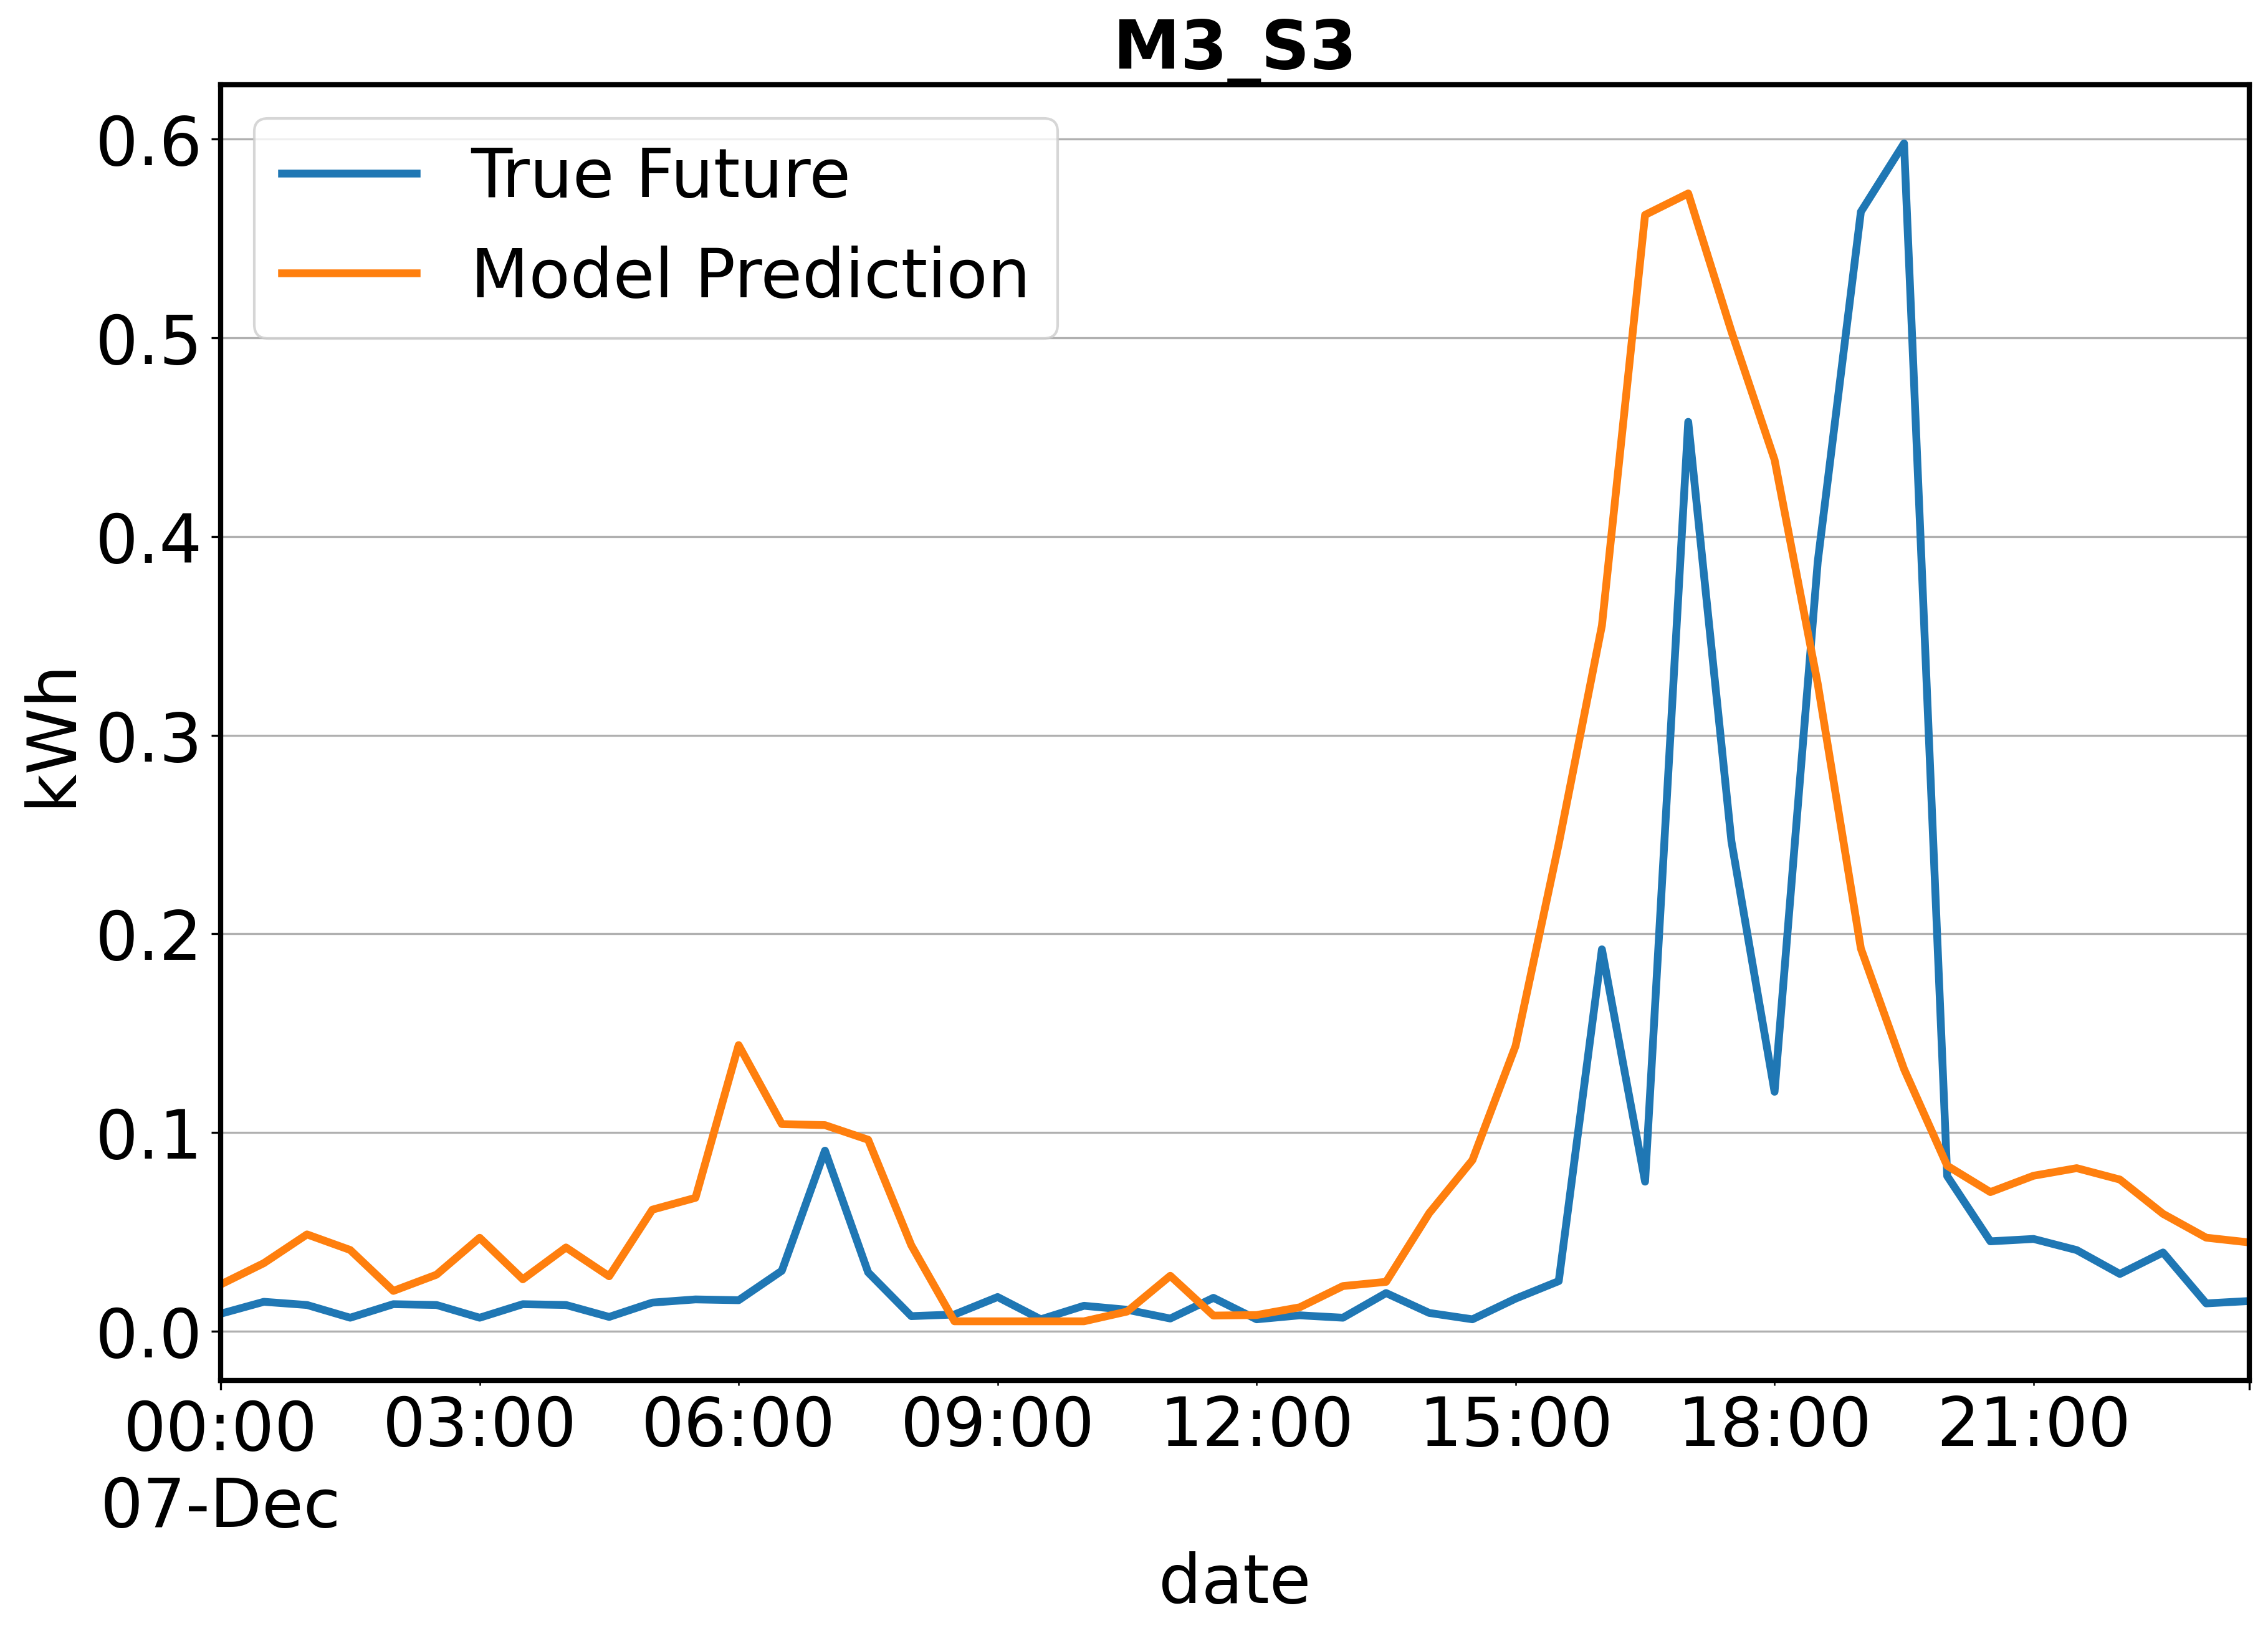
\includegraphics[width=1\linewidth]{IDM3_S3_Day341.png}
		\caption{Model $3 $ - Serie $ 3 $}
	\end{subfigure}
 	\begin{subfigure}{0.32\textwidth}
		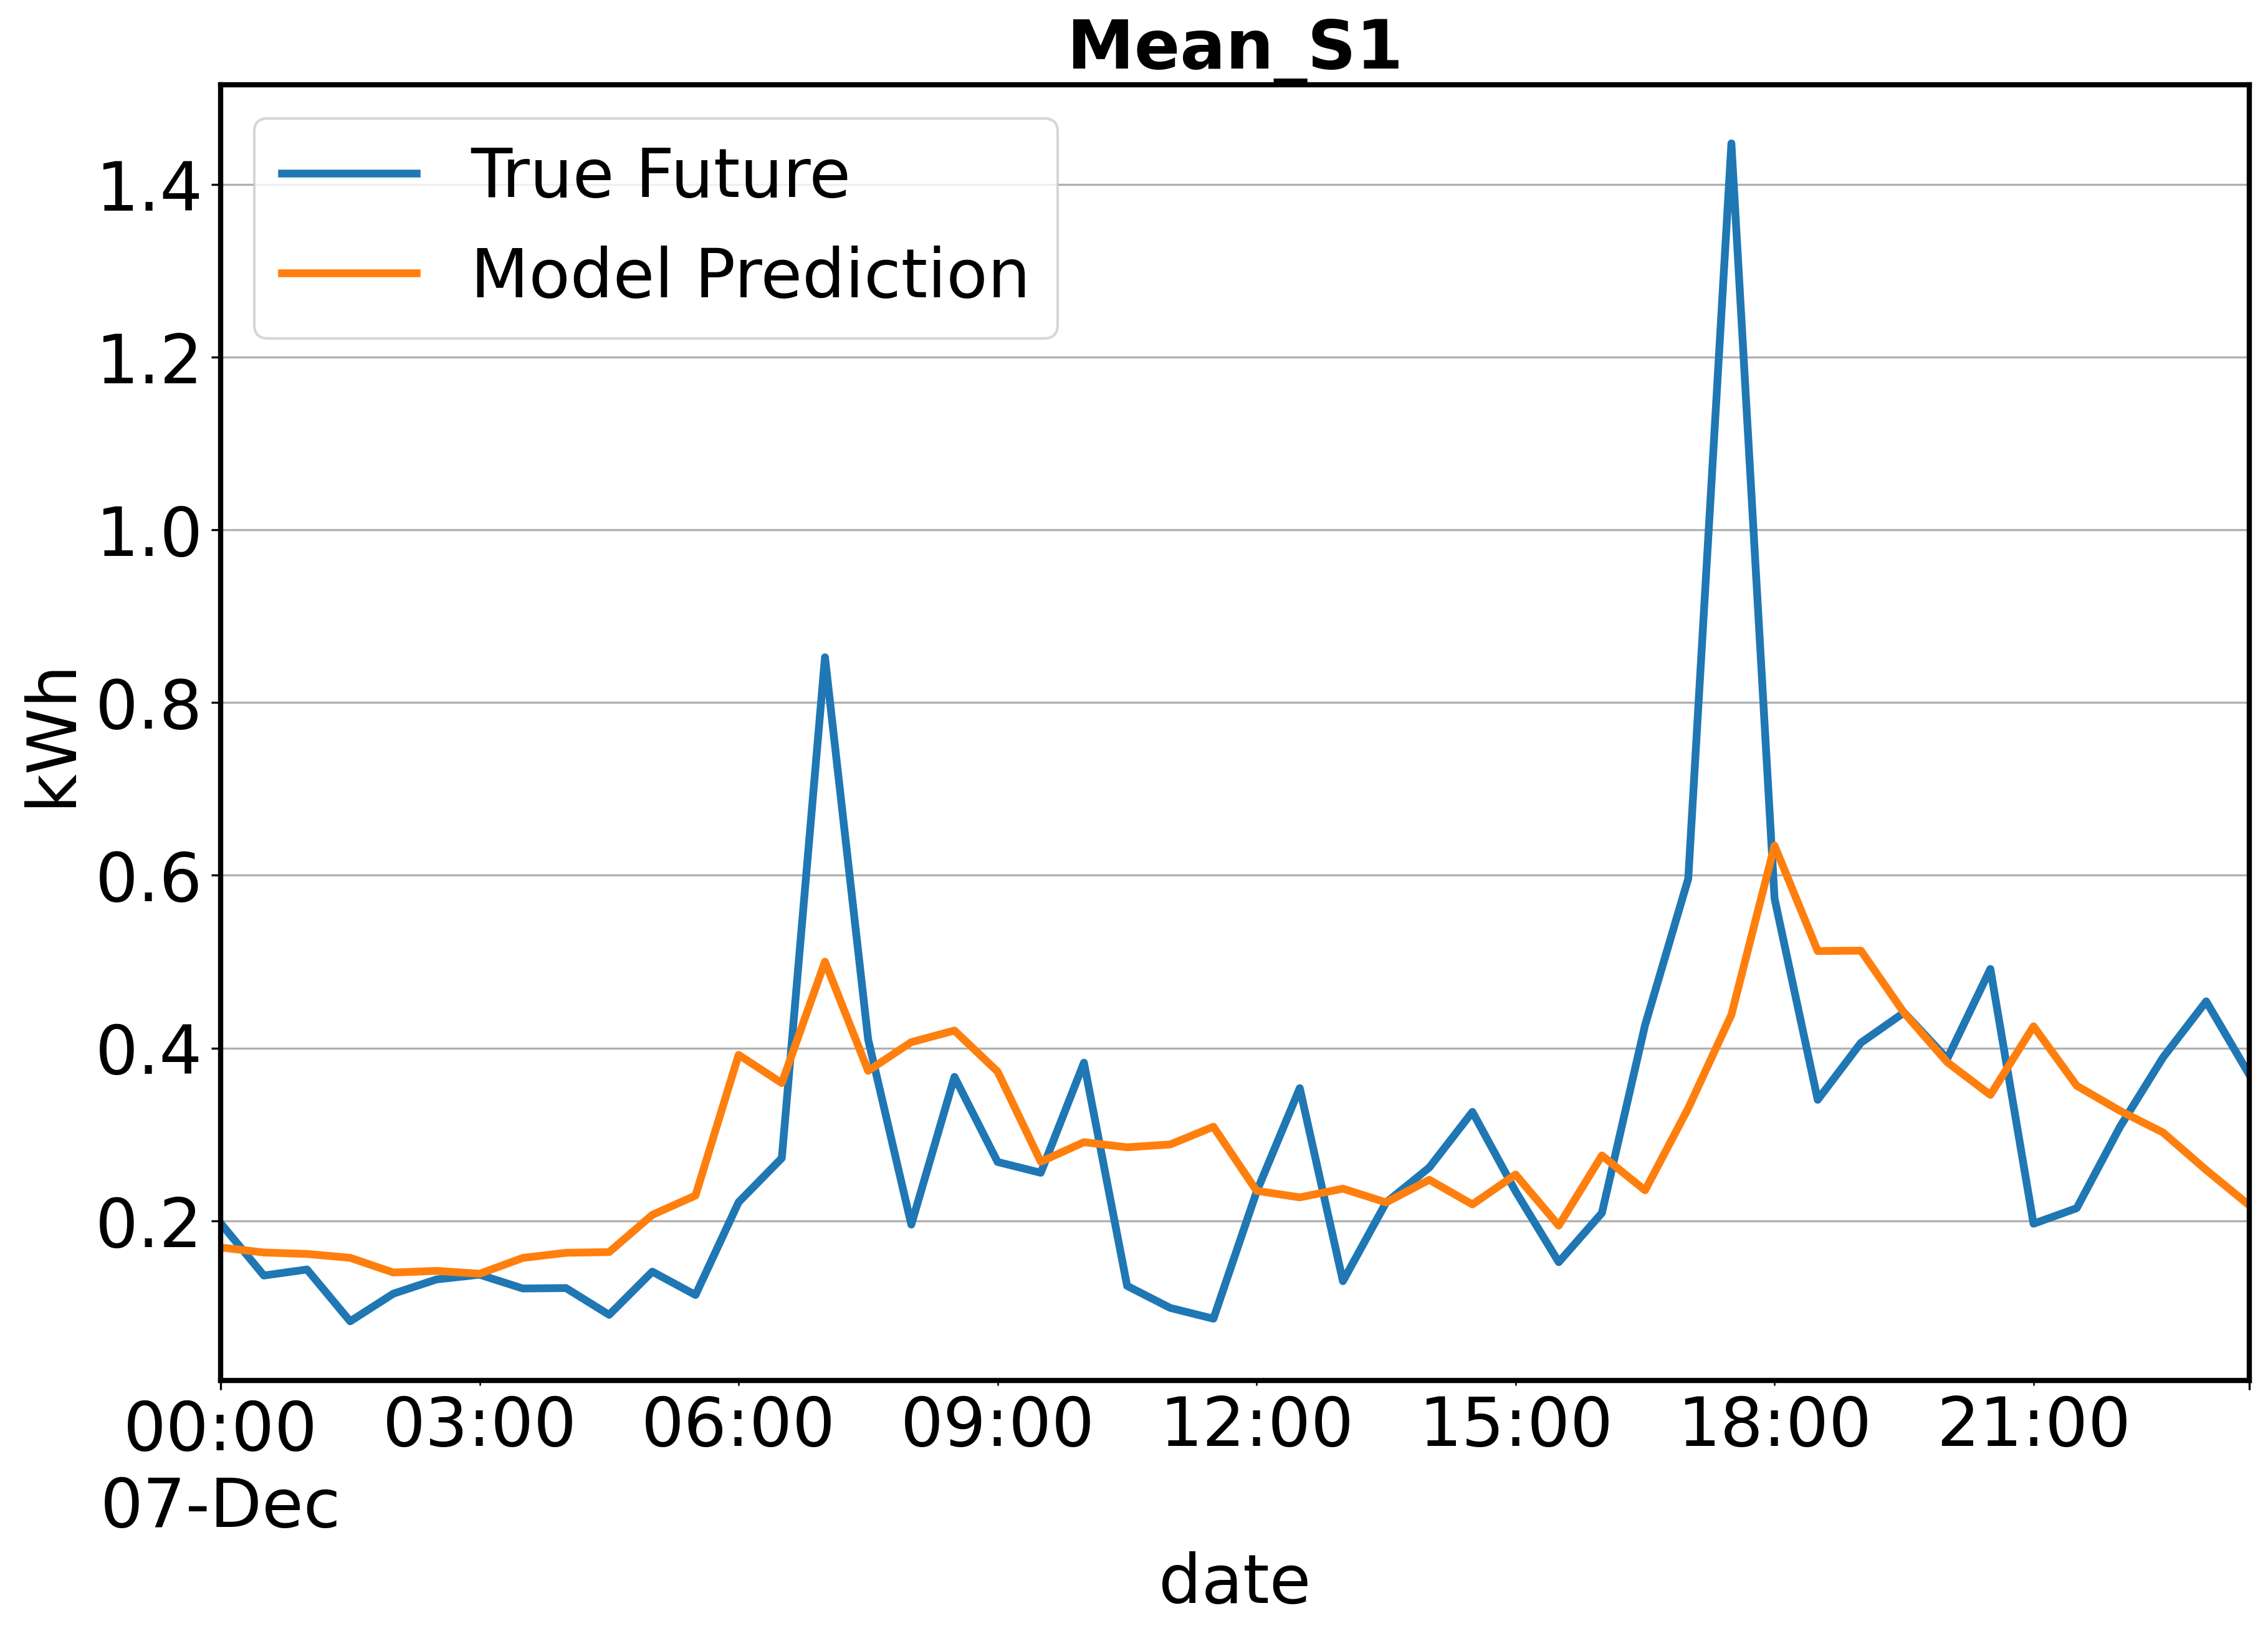
\includegraphics[width=1\linewidth]{IDMean_S1_Day341.png}
		\caption{Mean forecast - Serie $ 1 $}
	\end{subfigure}	 	
	\begin{subfigure}{0.32\textwidth}
		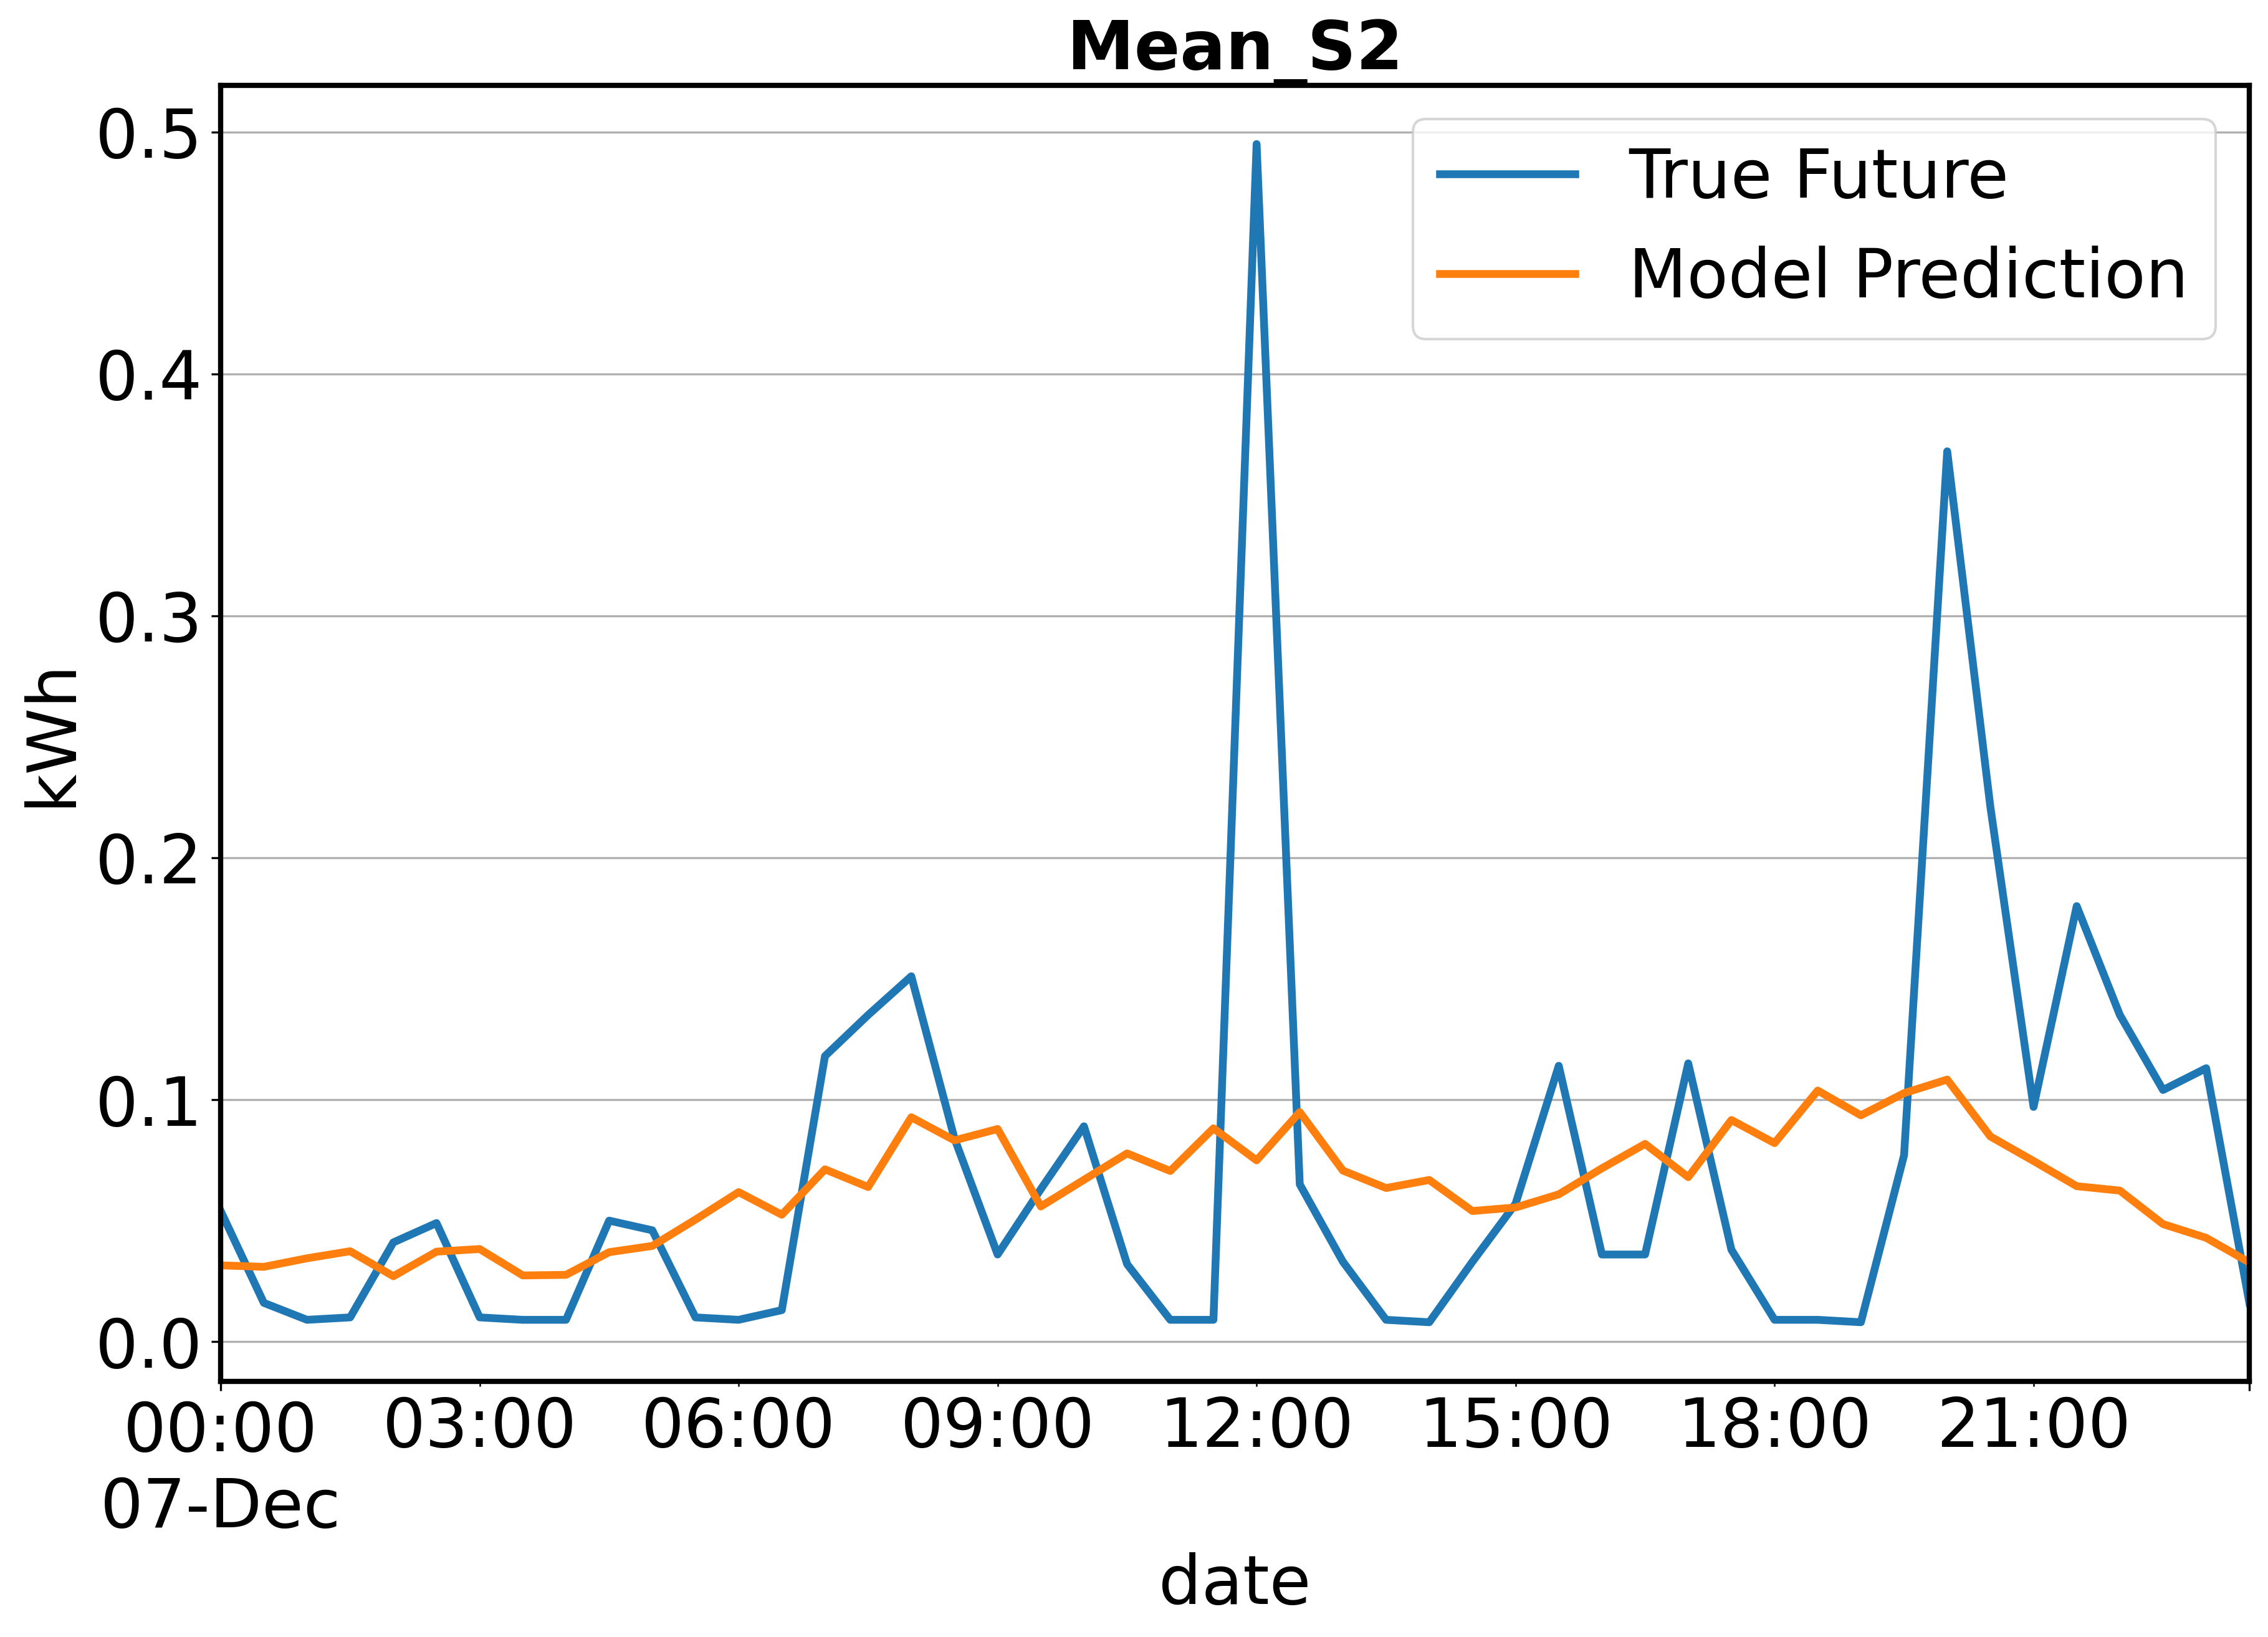
\includegraphics[width=1\linewidth]{IDMean_S2_Day341.png}
		\caption{Mean forecast - Serie $ 2 $}
	\end{subfigure}	
	\begin{subfigure}{0.32\textwidth}
		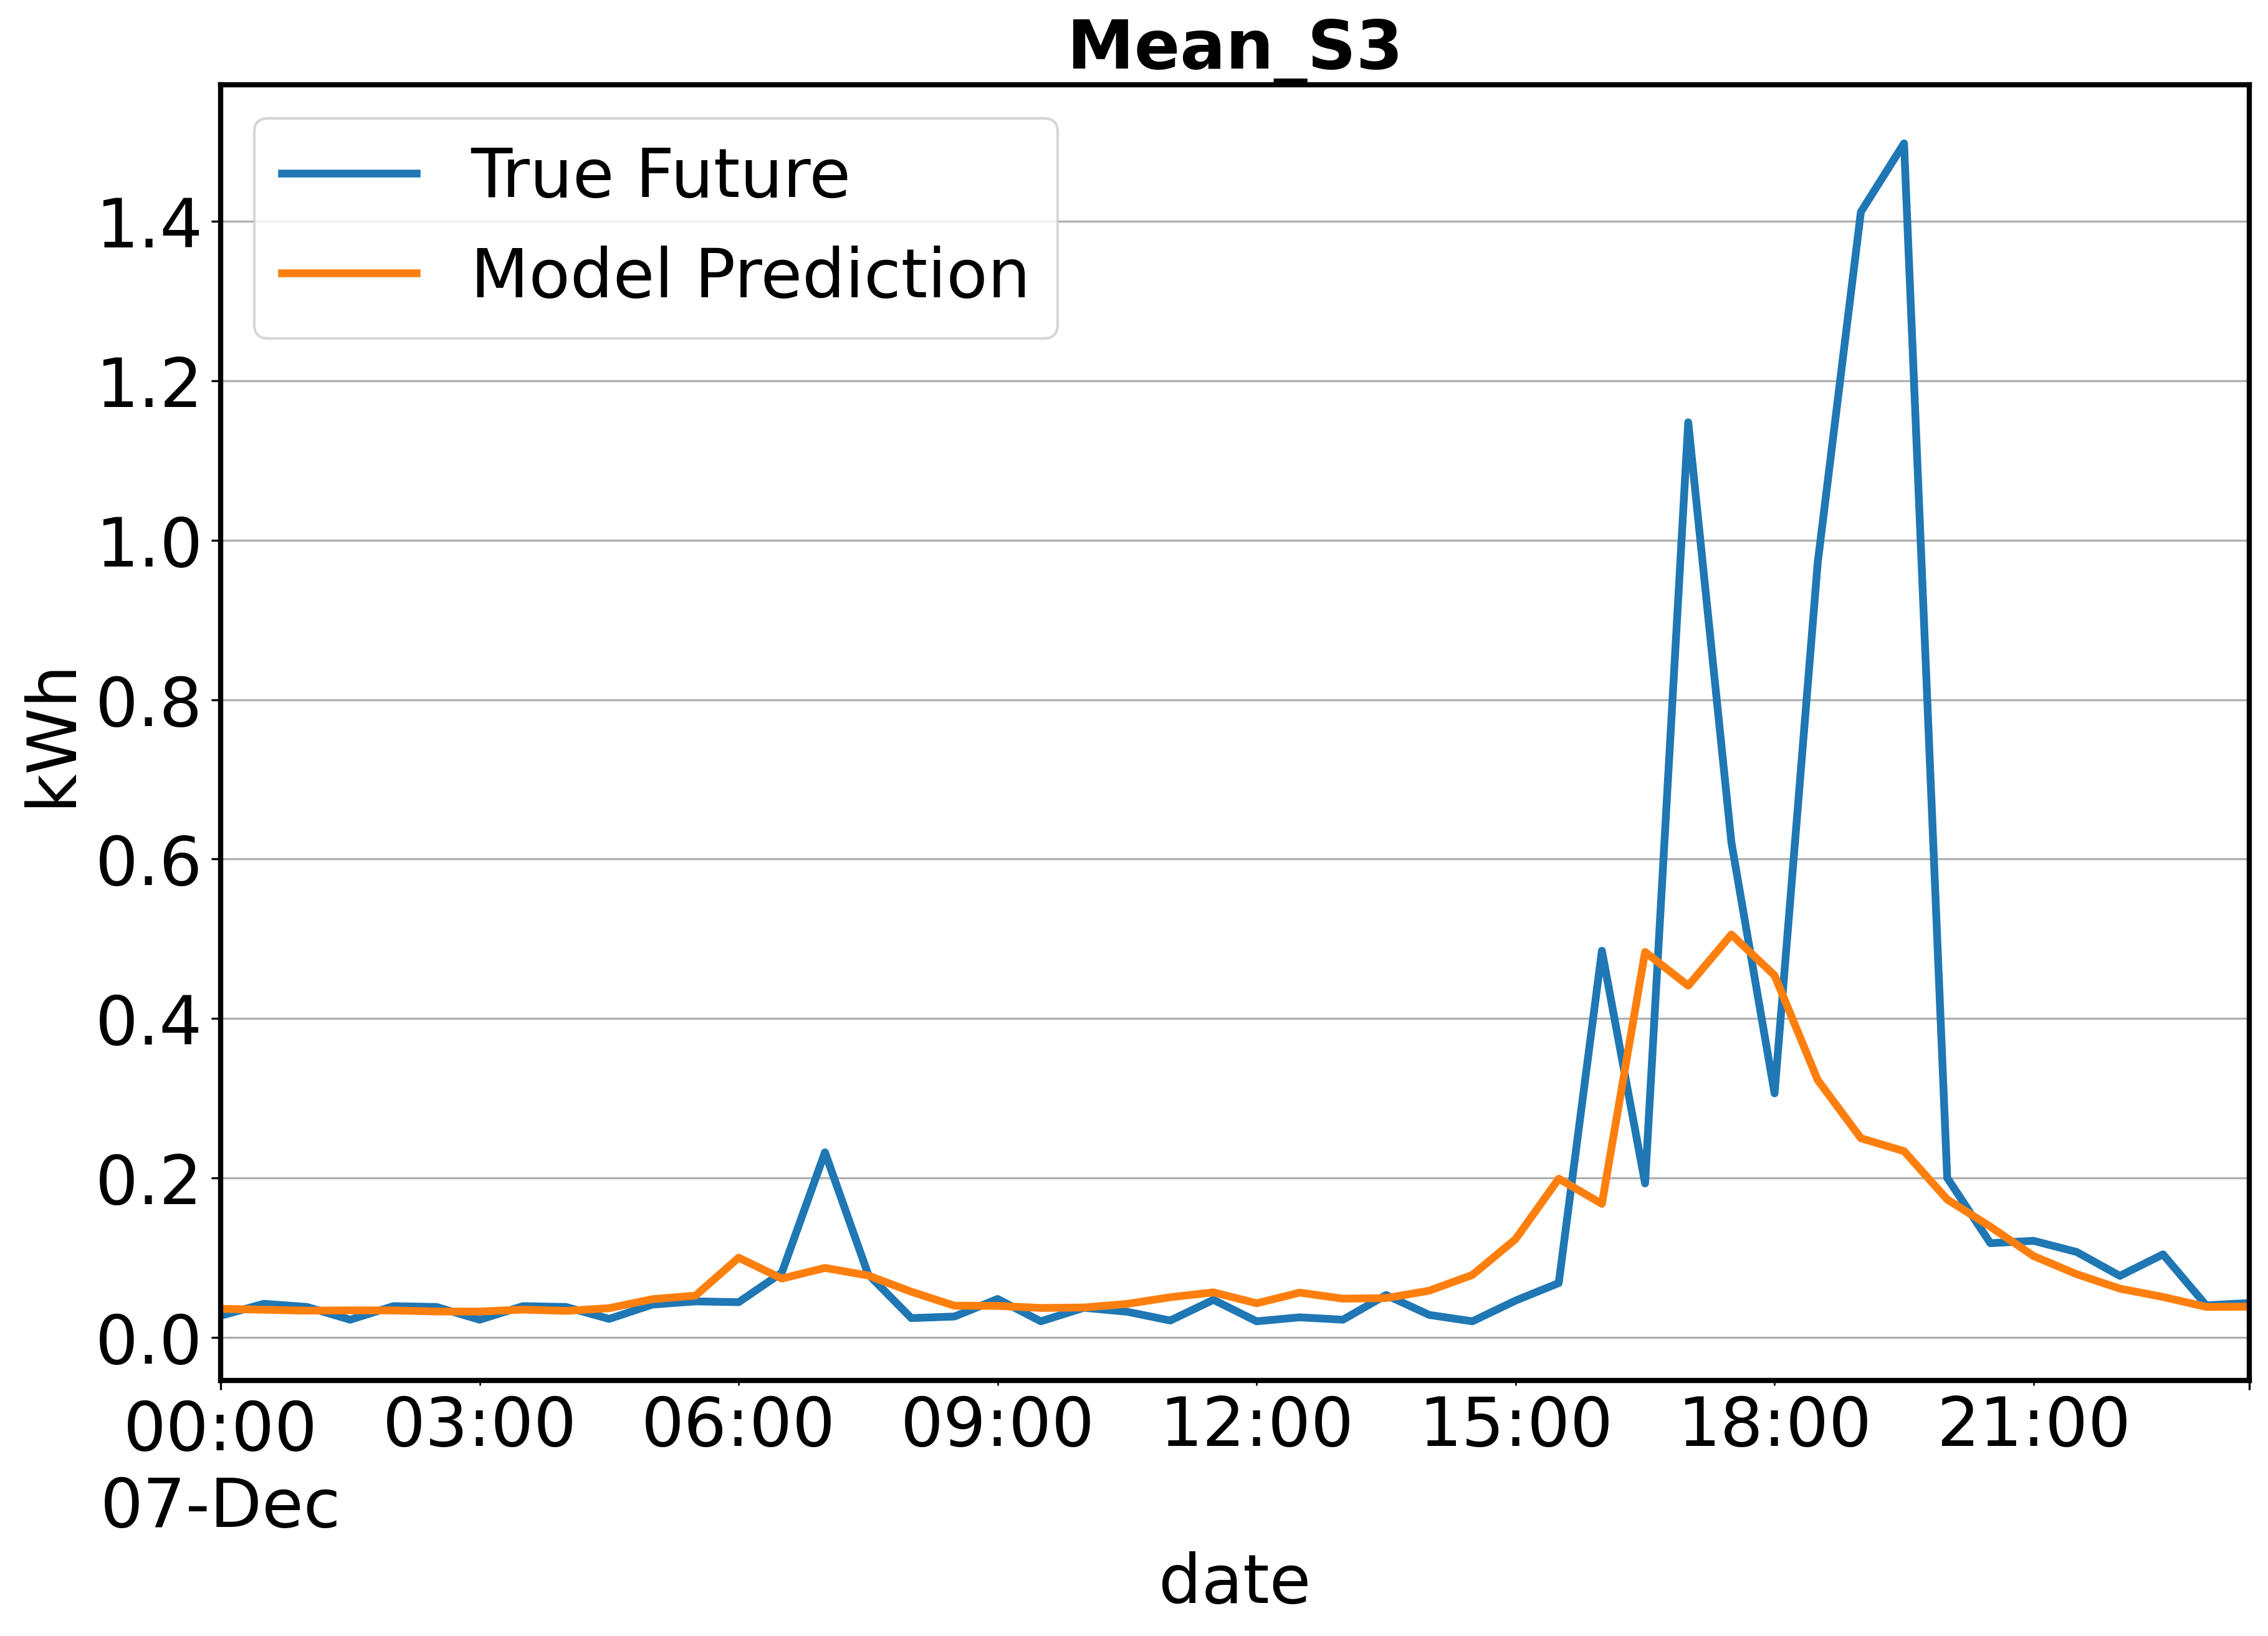
\includegraphics[width=1\linewidth]{IDMean_S3_Day341.png}
		\caption{Mean forecast - Serie $ 3 $}
	\end{subfigure}
	 \begin{subfigure}{0.32\textwidth}
		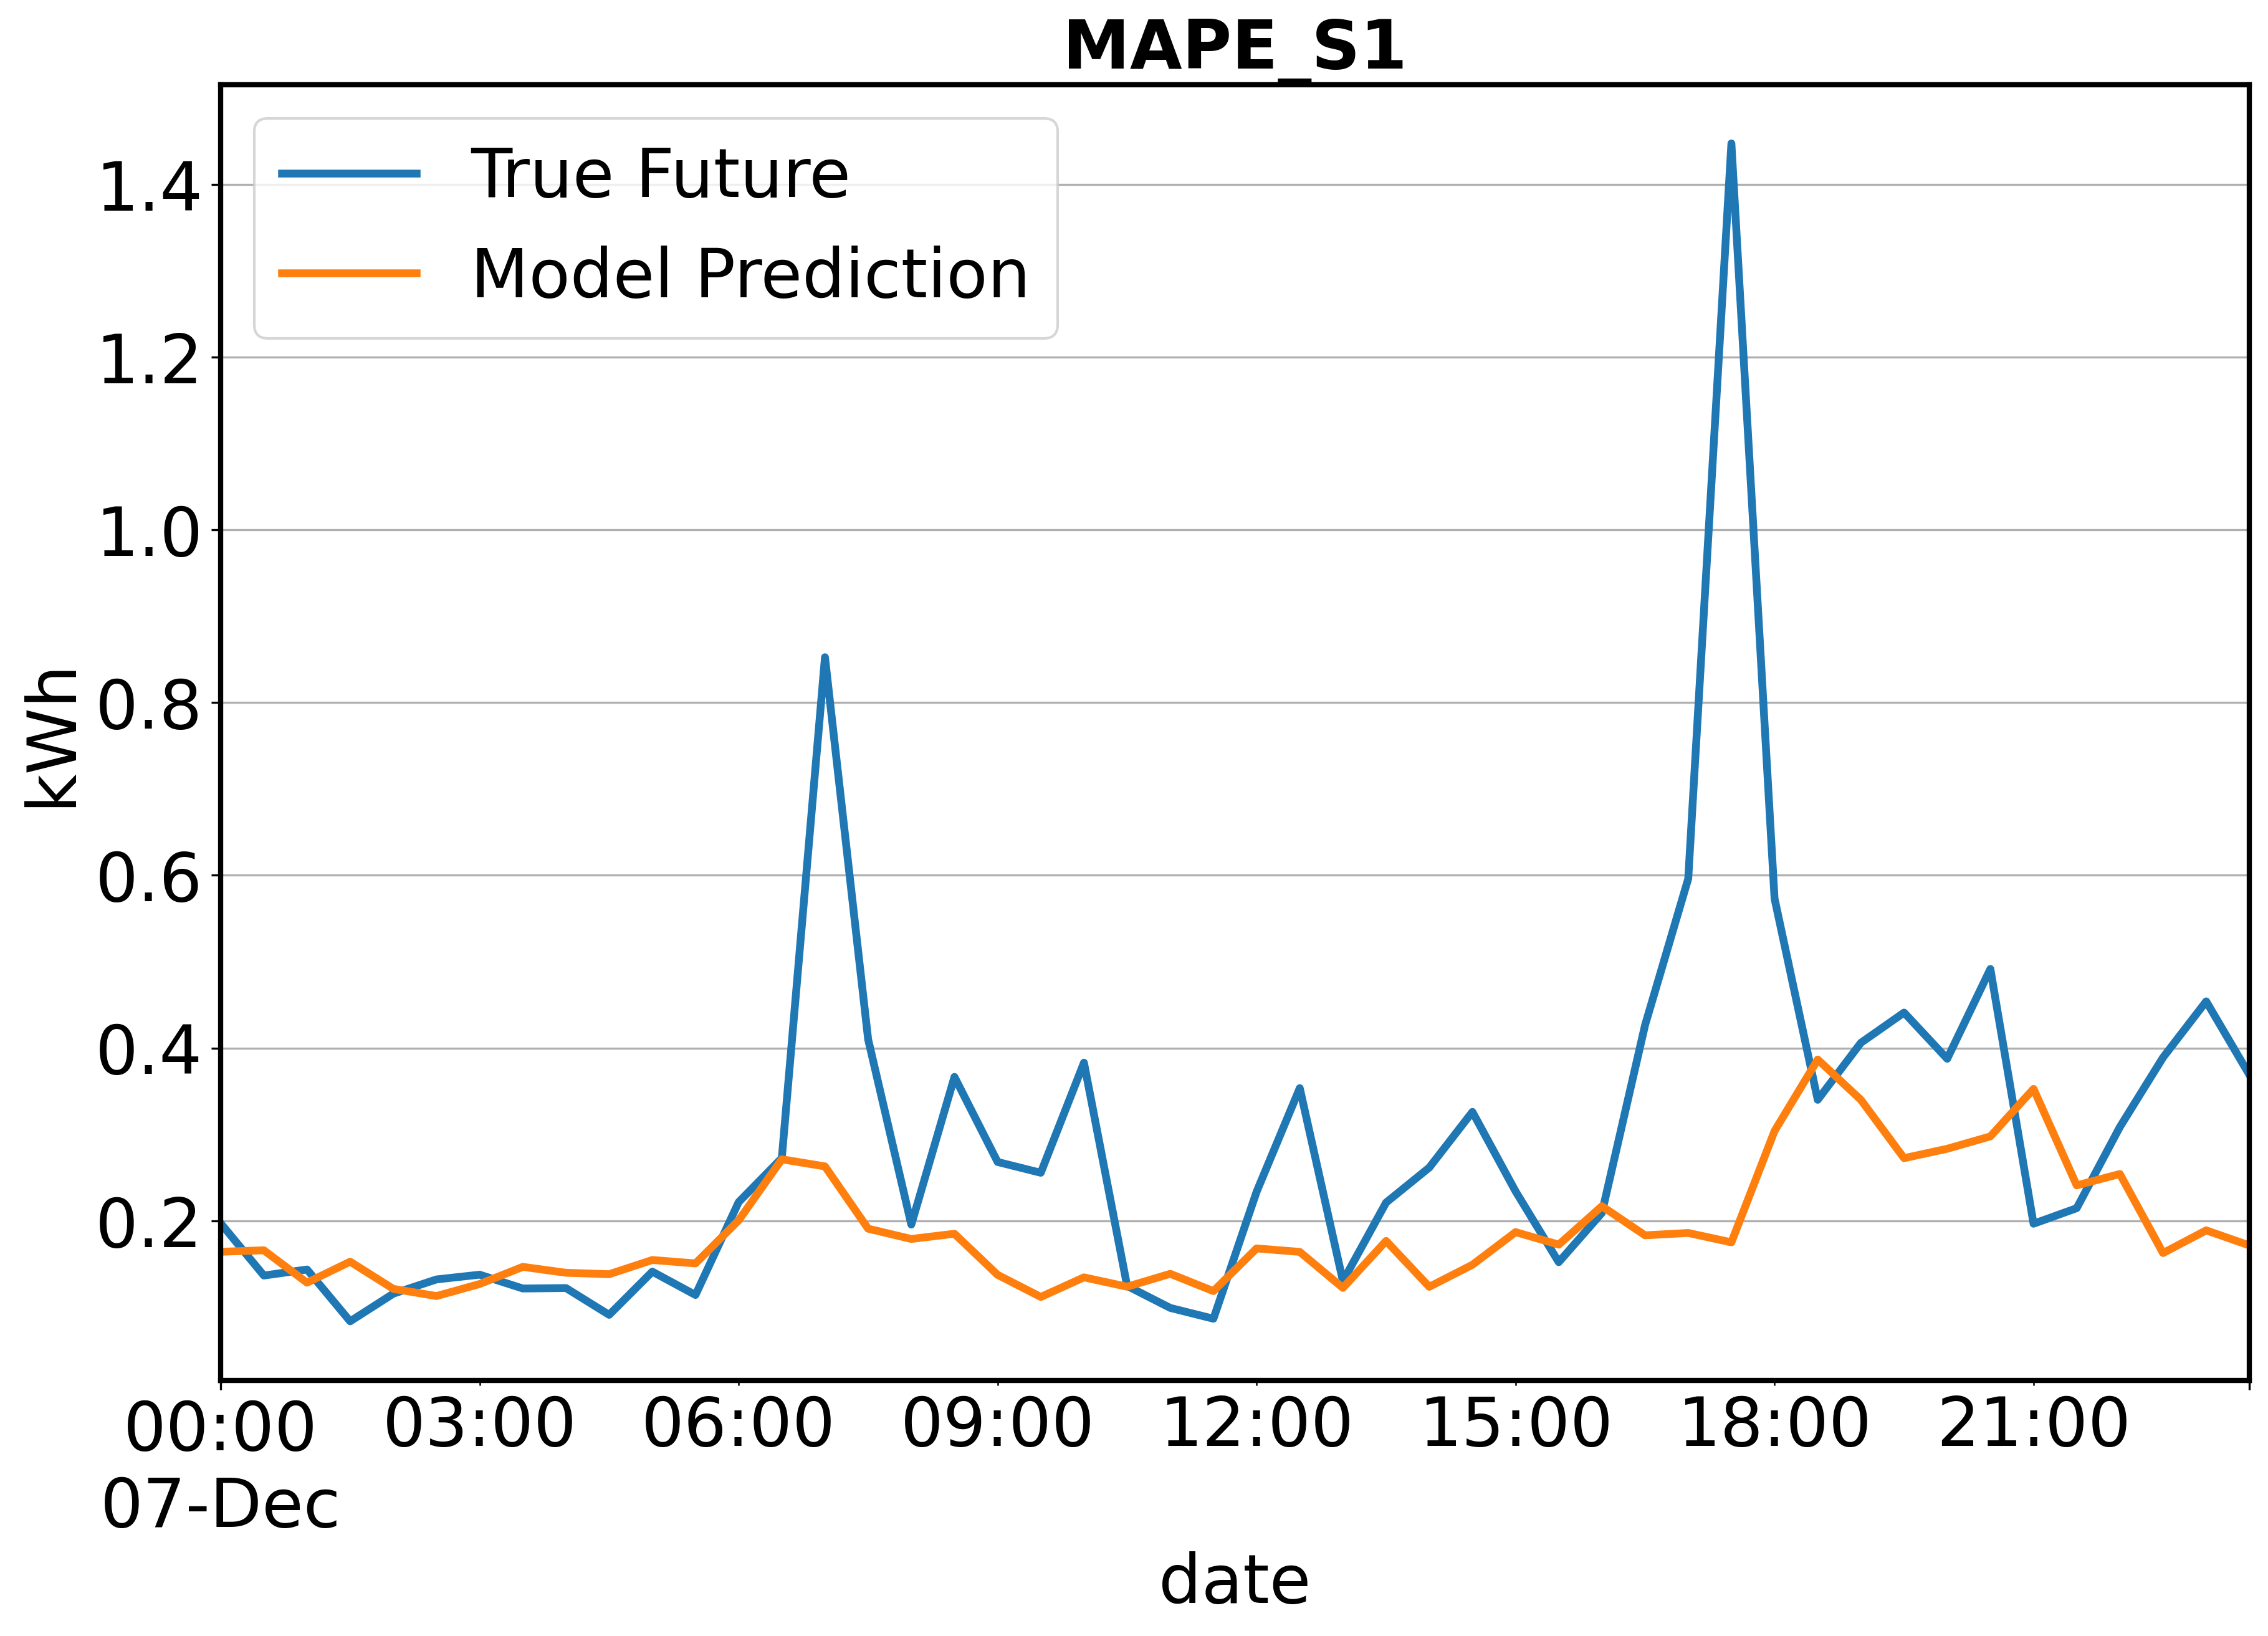
\includegraphics[width=1\linewidth]{IDMAPE_S1_Day341.png}
		\caption{MAPE forecast - Serie $ 1 $}
	\end{subfigure}	 	
	\begin{subfigure}{0.32\textwidth}
		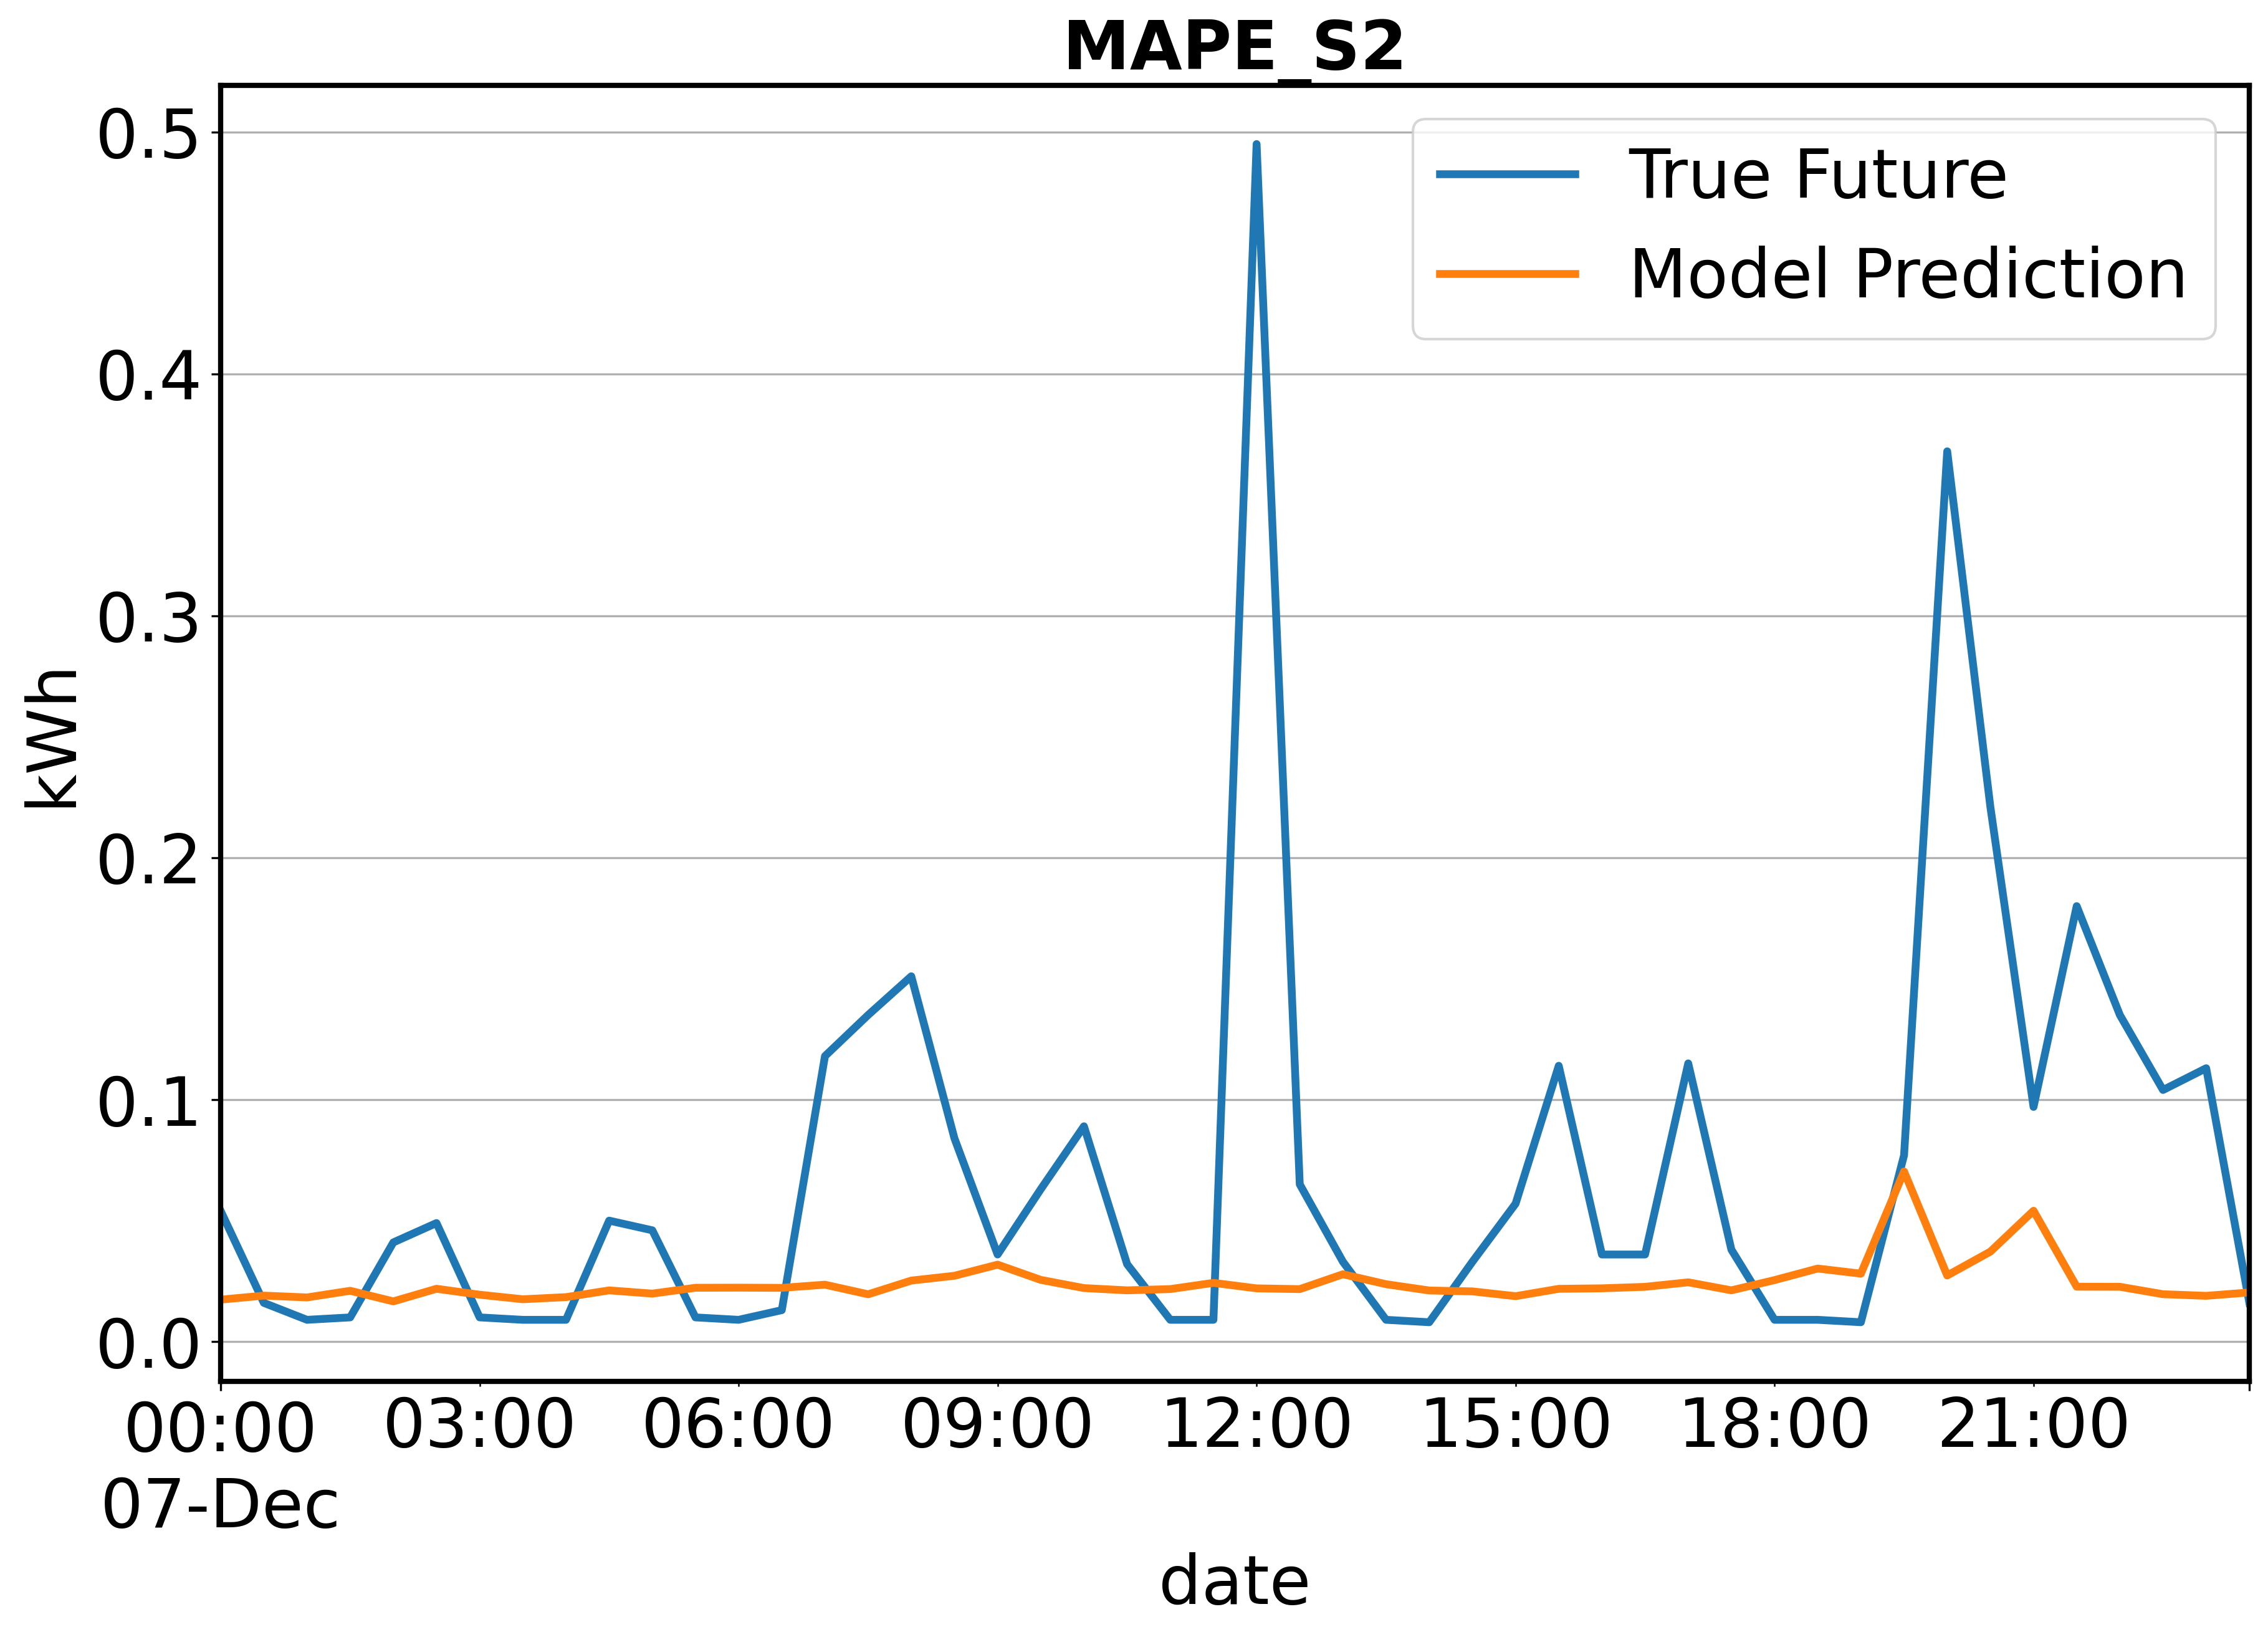
\includegraphics[width=1\linewidth]{IDMAPE_S2_Day341.png}
		\caption{MAPE forecast - Serie $ 2 $}
	\end{subfigure}	
	\begin{subfigure}{0.32\textwidth}
		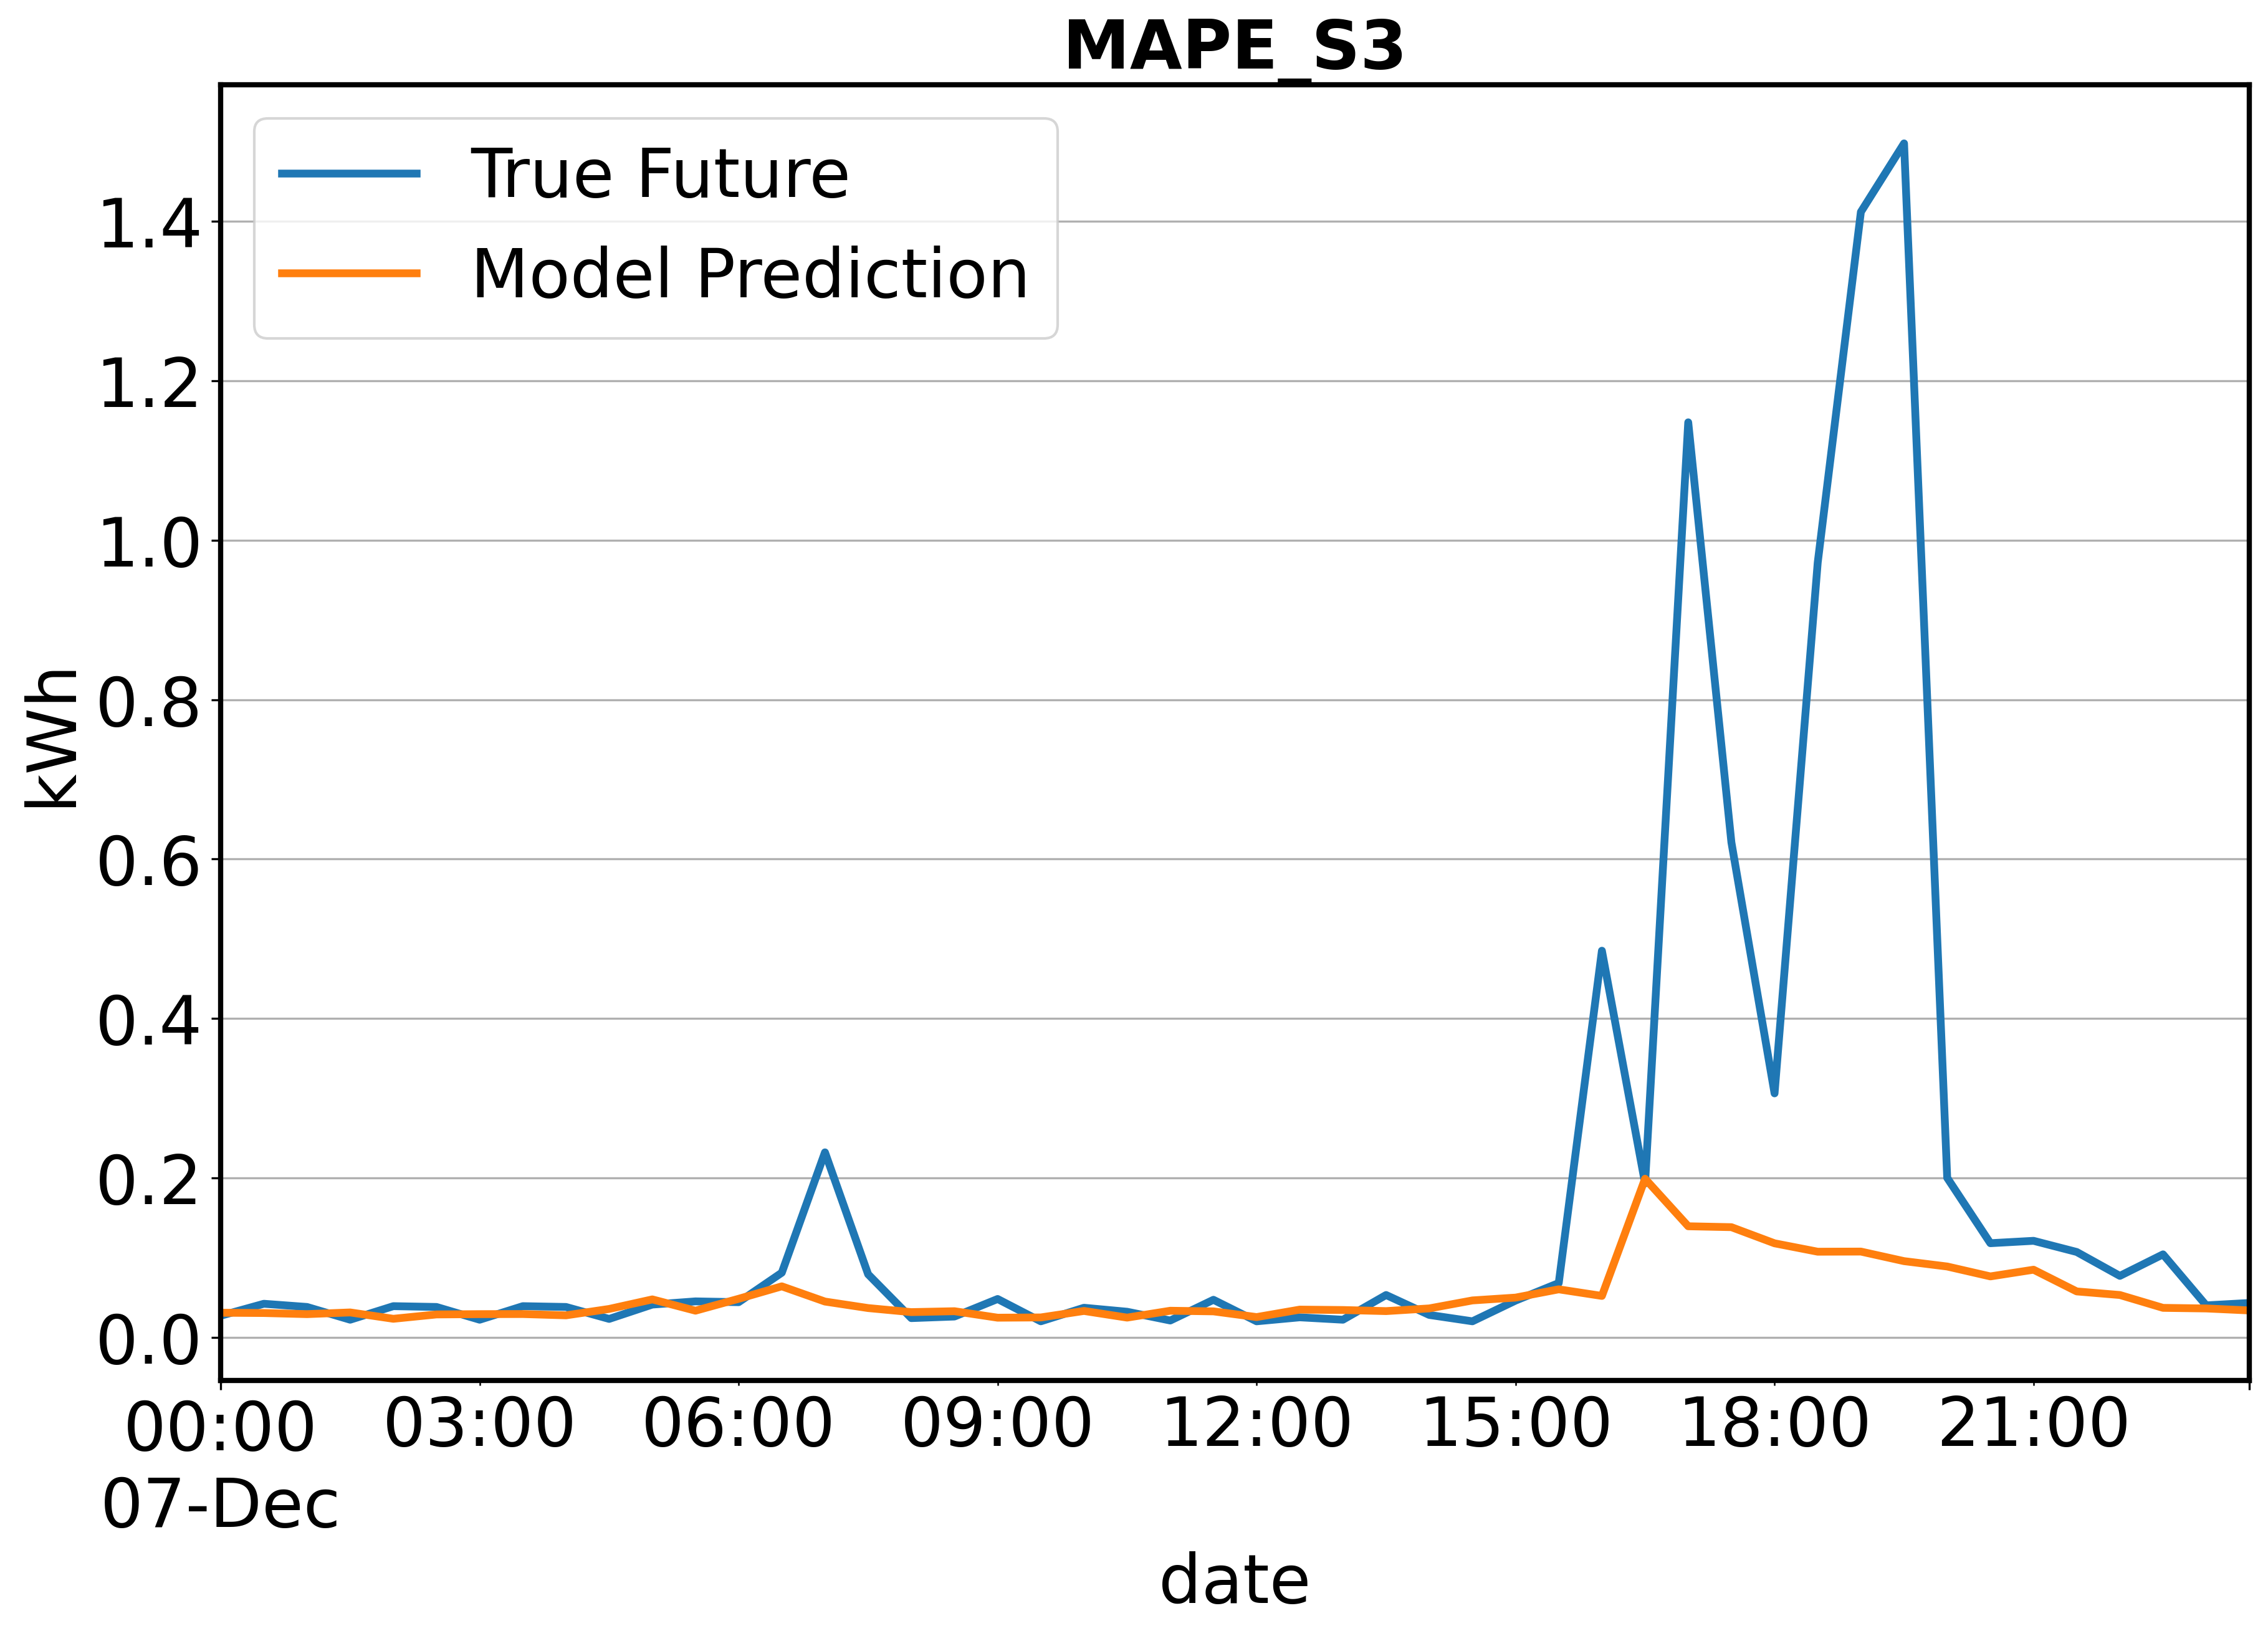
\includegraphics[width=1\linewidth]{IDMAPE_S3_Day341.png}
		\caption{MAPE forecast - Serie $ 3 $}
	\end{subfigure}
 	\caption{The prediction result of the different models on $ 7 $ December. (True Future: blue/ Prediction: orange)}
 	\label{fig:individual_forecasts}
 \end{figure}

- because makes use of MSE --> error is more focussed on forecasting the peaks.
- when would optimize for minimizing the MAPE error, the low consumptions would be the focus to forecast well because of the division by a small value what will cause a large error as given by: $ \hat{y}_t-y_t}/y_t$.

- It can be seen that the mean forecast can also capture the two peaks for Serie 1 and the single peak for Serie3, but as expected from an average the peaks are smaller. 

- clearly a difference when a regulation is added or not -- > for serie 3 both model 2 and model 3 see a small peak before the bigger peak. While model three produces a choppy peak, model two gives a much smoother peak. Another example is that model 1 and model 3 show a much more serrated signal than model two and serie one where regulation is added.

- 

It can be seen in Figure \ref{fig:individual_forecasts} but also in the other predicted days in the test set that especially at the beginning, there is a big offset between the predicted and reference signal when the LSTM models predict Serie 1. However, the peaks itself are present in about the right spot.

- the MAPE models are focussed on predicting the small values and therefore ignores all the peaks.





- see also notes from mail to Lola. 

Say that here use the models that obtained in the previous chapter. Make MSE plot for the different NN and the baseline models for each serie and make a comparison of the MAPE with the other baseline model. (by making use of barplots --> normalized with the worst performer) Performance on the test set. 

Make a plot of the day forecast for each NN model --> four graphs bundled. 
- for comparing performance in the same time serie --> mae is used. To compare performance between different time series --> MAPE is used. 
- for stateless random 10 percent is used as validation set. Remember that should shuffle the training set beforehand otherwise j
- for stateful --> the last 30 days of November will be used --> no shuffling is allowed.

- make a graph which shows all the different days that have to be forecasted on the x-axis and the MAE error on the y-axis for the different models. (line graph)

- give an indication how long the models trained --> amount of epochs. 

- when there are a lot of missing days in the test data: serie 1 (0 days) and the other two (8days) -->it is naturally that the model performs worse, the previous day it bases its forecast on is just an estimate. For the day that is forecasted are always days where the true reference signal is available. 



- bar plot for general performance (MAE and MAPE - basemodels and NN)

- line plot for the error on each day (MAE and MAPE - basemodels and NN)

- the signal for the forecast of a day for each model

- in some plots will see that there are gaps --> reason is that it is not useful to predict on the $ 8 $ missing days in the test set. There will only be an estimated signal available to calculate an error on. 

- the line plot shows the distribution of the error per day on the predictions per day. 

- also the mape metric is considered because it allows to compare between different series. 


\section{Conclusion}


%%% Local Variables: 
%%% mode: latex
%%% TeX-master: "thesis"
%%% End: 
